\section{Action Phase: 3D Renderer}


\subsection{Big Picture}

During action sequences, the 3D scene is rendered in four passes:
\begin{enumerate}
 \item Clear the screen by drawing the floor and the ceiling (both solid color).
 \item Cast up to 320 rays and draw then according to the distance from the player.
 \item Draw the things (enemies, lamps, barrels).
 \item Draw the weapon.	
\end{enumerate}

Assets come from file VMSWAP:
\begin{enumerate}
	\item Textures for the wall are stored uncompressed.
	\item Sprites are ...They are not compressed per say but because they contain a lot of optimization: Own many columns to skip on the left. How wide they are. Since scprite are drawn as column....chunk offsets ahd chunk length. Sprites are drawn bottom up
\end{enumerate}
Following, screenshots of a slowdown version of the engine, showing each four step of rendition:
\begin{figure}[H]
\centering
 
\includegraphics[width=\textwidth]{screenshots/wolf3d_1_background.png}
 \caption{3D Rendere Phase 1: Background}
 \end{figure}
The floor was always the same color. The ceiling however changed see \codeword{WL\_DRAW.C} for a hard-coded index. TODO: Include a clear screen from a later level.\\
\begin{figure}[H]
 \centering
  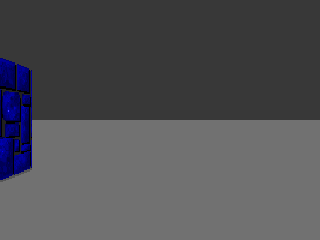
\includegraphics[width=\textwidth]{screenshots/wolf3d_4_partial_wall_32rays.png}
  \caption{3D Rendere Phase 2: Walls (160 rays)}
 
\end{figure}
 
\begin{figure}[H]
 \centering
  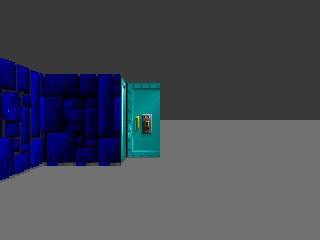
\includegraphics[width=\textwidth]{screenshots/wolf3d_5_partialwalls_160rays.png}
 \caption{Finalez frame} 
 
\end{figure}
 
 
 \begin{figure}[H]
\centering
 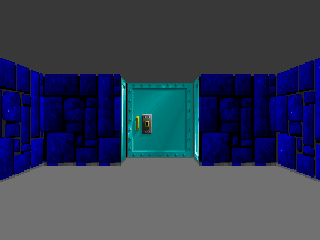
\includegraphics[width=\textwidth]{screenshots/wolf4d_2_walls.png}
 \caption{3D Rendere Phase 2: Walls completed} 
 \end{figure}
 
 
 \begin{figure}[H]
\centering
 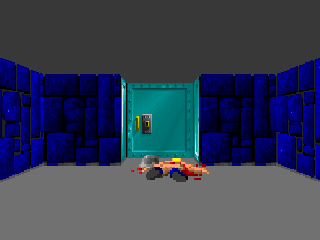
\includegraphics[width=\textwidth]{screenshots/wolf3d_6_scaled}
 \caption{3D Rendere Phase 3: Scaled (a.k.a: Sprites)} 
 \end{figure}

 \begin{figure}[H]
\centering
 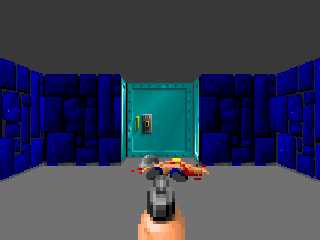
\includegraphics[width=\textwidth]{screenshots/wolf3d_7_fullframe.png}
 \caption{3D Rendere Phase 2: Weapon} 
 \end{figure}
 

   Synergy: VGA column drawing, raycasting, occlusion array\\


The static part (ammo, face, etc) is not redrawn if not necessary. However cost is high since the new part of the screen has to be draw in three buffers (e\.g:StatusDrawPic) .










\subsection{HUD}
\begin{figure}[H]
  \centering
 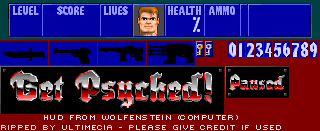
\includegraphics[width=\textwidth]{imgs/sprites.png}
\end{figure}









\subsection{Clearing the screen}






\subsection{Casting a Ray}

\subsubsection{Fixed point}
The hardware chapter describing the CPU capabilities left the reader with a problem at hands: The machine cannot do floating point operations fast enough. This is a pretty big deal for a 3D engine and all the trigonometry involved. It turns out the solution is to trick the ALU via a technique called "fixed point arithmetic":\\
\par
The nomal layout of an \cw{int} is as follow:
\begin{figure}[H]
\centering
 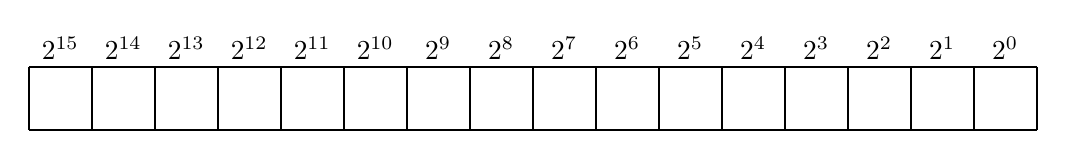
\begin{tikzpicture}[scale=0.8, every node/.style={scale=0.99}]
\draw[thick] (0,0) -- (16,0);
\draw[thick] (0,1) -- (16,1);
\foreach \i in {0,...,16}
{
     \draw[thick] (\i,1) -- (\i,0);
}

\foreach \i in {0,...,15}
{
     \node[] at (15-\i+0.5,1.3){$2^{\i}$}  ;
       
       
     
}
\end{tikzpicture}

 \caption{Integer layout.} \label{fig:int_layout}
 \end{figure}
The value of the sequence of bits \emph{0010010010010010}:
\begin{figure}[H]
\centering
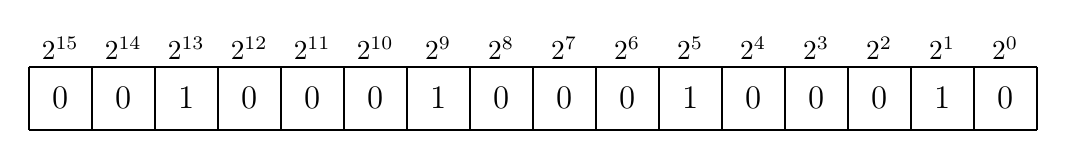
\begin{tikzpicture}[scale=0.8, every node/.style={scale=0.99}]
\draw[thick] (0,0) -- (16,0);
\draw[thick] (0,1) -- (16,1);
\foreach \i in {0,...,16}
{
     \draw[thick] (\i,1) -- (\i,0);
}

\foreach \i in {0,...,15}
{
     \node[] at (15-\i+0.5,1.3){$2^{\i}$}  ;
}

\tikzstyle{fontbf} = [font=\large]
\node[fontbf] at (0.5,0.5){0} ;
\node[fontbf] at (1.5,0.5){0};  
\node[fontbf] at (2.5,0.5){1} ; 
\node[fontbf] at (3.5,0.5){0} ;

\node[fontbf] at (4.5,0.5){0} ;
\node[fontbf] at (5.5,0.5){0};  
\node[fontbf] at (6.5,0.5){1} ; 
\node[fontbf] at (7.5,0.5){0} ;

\node[fontbf] at (8.5,0.5){0} ;
\node[fontbf] at (9.5,0.5){0};  
\node[fontbf] at (10.5,0.5){1} ; 
\node[fontbf] at (11.5,0.5){0} ;

\node[fontbf] at (12.5,0.5){0} ;
\node[fontbf] at (13.5,0.5){0};  
\node[fontbf] at (14.5,0.5){1} ; 
\node[fontbf] at (15.5,0.5){0} ;


\end{tikzpicture}

 \caption{Integer example.} \label{fig:mips}
 \end{figure}

 Is equal to $ 2^{13} + 2^9 + 2^5 + 2^1 =  8738 $.\\
 \par

Fixed Point allows to keep track of fractions while still using the integer operations of the CPU. The machine manipulates what are supposed to be integer numbers but the programmers sees them as a value containing an integer part and a fractional part:\\
\par
\begin{figure}[H]
 \centering
  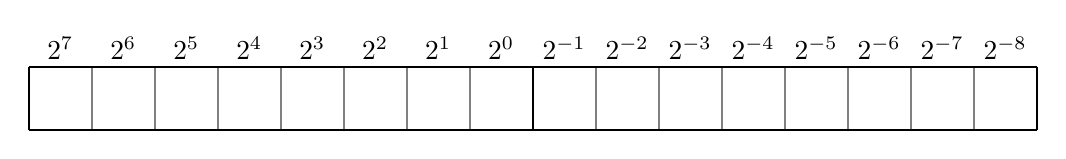
\begin{tikzpicture}[scale=0.8, every node/.style={scale=0.99}]


\colorlet{LighterMark}{black!50}

\foreach \i in {1,...,15}
{
     \draw[thick,LighterMark] (\i,1) -- (\i,0);
}

     \draw[thick,black] (0,1) -- (0,0);
      \draw[thick,black] (8,1) -- (8,0);
      \draw[thick,black] (16,1) -- (16,0);
      
\draw[thick,black] (0,0) -- (16,0);
\draw[thick,black] (0,1) -- (16,1);
 

%\foreach \i[evaluate={\pow=int(7-\i)}] in {0,...,7}
\foreach \i[evaluate={\pow=int(7-\i)}] in {0,...,7}
{
   \node[] at (\i+0.5,1.3){$2^{\pow}$  }  ;
      
         
     
}

%\foreach \i[evaluate={\pow=int((\i-7)*2)}]  in {8,...,15}
\foreach \i[evaluate={\pow=int(\i-7)}]  in {8,...,15}
{
     \node[] at (\i+0.5,1.3){$2^{-\pow}$}  ;
}




\end{tikzpicture}

 \caption{Fixed point layout 8:8 (8bits for integer part and 8 bits for fractionnal part).} \label{fig:mips}
\end{figure}

So the same sequence of bits \emph{0010010010010010}:
\begin{figure}[H]
 \centering
   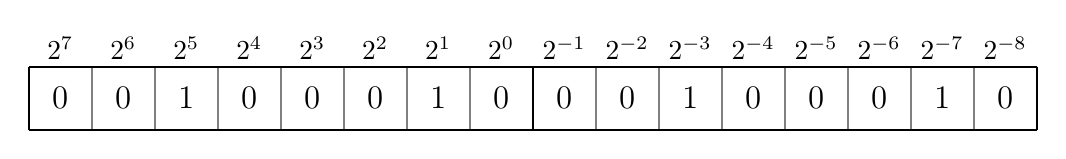
\begin{tikzpicture}[scale=0.8, every node/.style={scale=0.99}]


\colorlet{LighterMark}{black!50}

\foreach \i in {1,...,15}
{
     \draw[thick,LighterMark] (\i,1) -- (\i,0);
}

     \draw[thick,black] (0,1) -- (0,0);
      \draw[thick,black] (8,1) -- (8,0);
      \draw[thick,black] (16,1) -- (16,0);
      
\draw[thick,black] (0,0) -- (16,0);
\draw[thick,black] (0,1) -- (16,1);
 

%\foreach \i[evaluate={\pow=int(7-\i)}] in {0,...,7}
\foreach \i[evaluate={\pow=int(7-\i)}] in {0,...,7}
{
   \node[] at (\i+0.5,1.3){$2^{\pow}$  }  ;
      
         
     
}

%\foreach \i[evaluate={\pow=int((\i-7)*2)}]  in {8,...,15}
\foreach \i[evaluate={\pow=int(\i-7)}]  in {8,...,15}
{
     \node[] at (\i+0.5,1.3){$2^{-\pow}$}  ;
}

\tikzstyle{fontbf} = [font=\large]
\node[fontbf] at (0.5,0.5){0} ;
\node[fontbf] at (1.5,0.5){0};  
\node[fontbf] at (2.5,0.5){1} ; 
\node[fontbf] at (3.5,0.5){0} ;

\node[fontbf] at (4.5,0.5){0} ;
\node[fontbf] at (5.5,0.5){0};  
\node[fontbf] at (6.5,0.5){1} ; 
\node[fontbf] at (7.5,0.5){0} ;

\node[fontbf] at (8.5,0.5){0} ;
\node[fontbf] at (9.5,0.5){0};  
\node[fontbf] at (10.5,0.5){1} ; 
\node[fontbf] at (11.5,0.5){0} ;

\node[fontbf] at (12.5,0.5){0} ;
\node[fontbf] at (13.5,0.5){0};  
\node[fontbf] at (14.5,0.5){1} ; 
\node[fontbf] at (15.5,0.5){0} ;


\end{tikzpicture}

  \caption{Fixed point representation: 8738 is now 34.1328125.} \label{fig:mips}
\end{figure} 

Now represents:\\
\\
$ 2^5 + 2^1 = 34 $ for the integer part.\\
$ 2^{-3}+2^{-7} = 0.1328125 $ for the fractional part.\\
$ = 34.1328125$\\

\bigskip

The beauty of fixed point is that addition and subtraction work exactly like integers from the CPU instruction side:\\



\par
\begin{figure}[H]
  \centering
 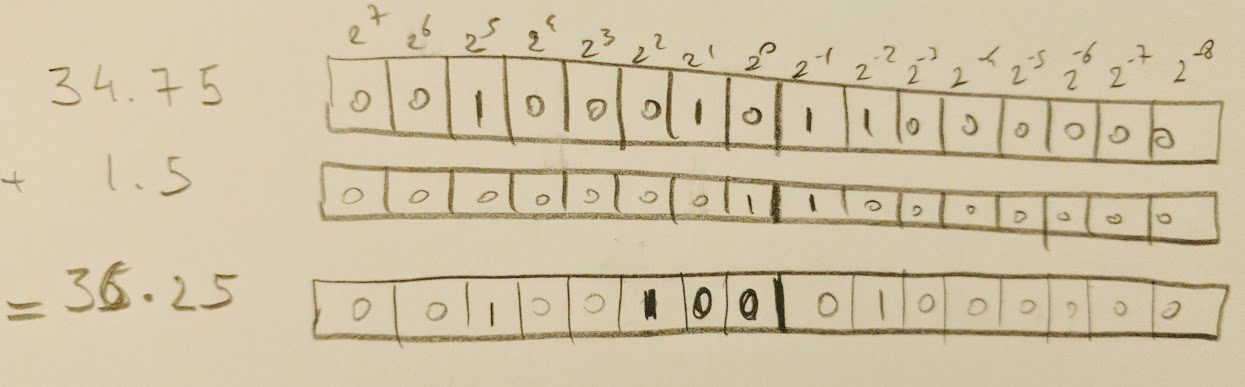
\includegraphics[width=\textwidth]{imgs/fixed_point_addition.png}
\end{figure}
\par


 The special case is when performing multiplication. There are two ways to do it: Either multiply two 32 bits into a 64 bits or drop the precision of both fixed point and multiply then into a 32 bits. Since the 286 and 386 do not have 64 bits registers, wolf does the later (illustred here with 8:8 for readability):

\par
\begin{figure}[H]
  \centering
 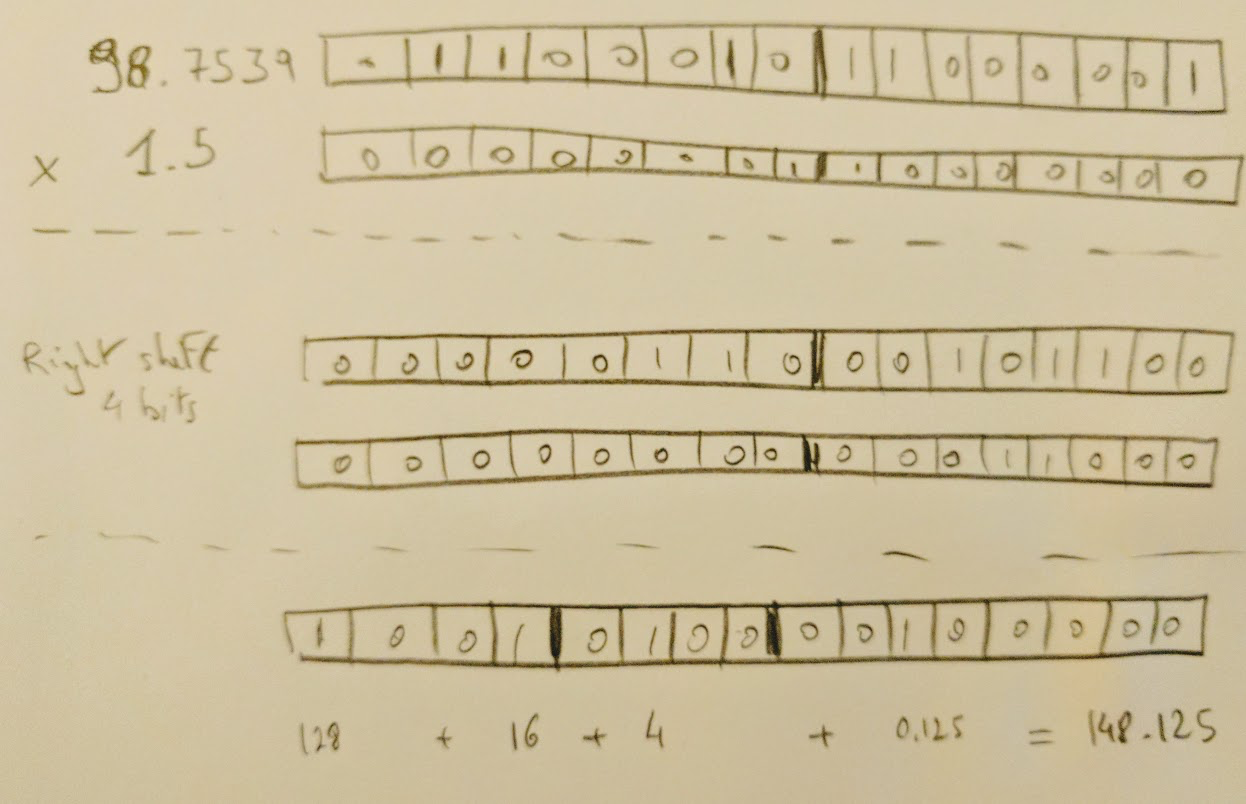
\includegraphics[width=\textwidth]{imgs/fixed_point_multiplication.png}
\end{figure}
\par

Notice that you have to be careful: In the previous example some precision was lost ($ 2^{-8}$) bit disappeared during the $\gg 4$ operation) and an overflow could have occured (multiplying by 3 would have gone past the precision of 8:8). But with this system, fractions are possible and fast enough!\\
\par

 \lstinputlisting[language=C]{code/fixed_mul.c}
\par
 \textbf{\underline{Trivia :}}  Fixed Point Arithmetic usage was not limited to PC gaming. Many game console manufactured in the 90s and later had no hardware floating point unit: Sony's original PlayStation (1994) and Sega's Saturn (1994) are examples among many with a design choice that not only reduced the production cost but also maximized the CPU pipeline throughput.
 
 Even right shit and left shift trick work:\\
 
\begin{figure}[H]
  \centering
 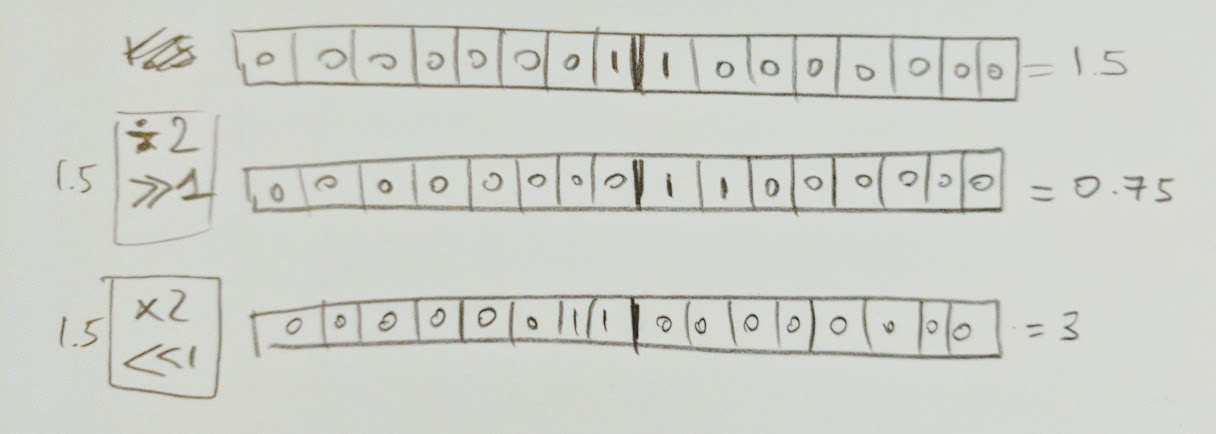
\includegraphics[width=\textwidth]{imgs/fixed_point_shifts.png}
\end{figure}
\par
 
 
 

\subsubsection{Square World and RayCasting}
With fraction possible, the engine still needs to find a way to render the walls in pseudo-3D. Per say, draw a wall bigger if it is closer and smaller if it is far. To do that, it cast a ray for each column of pixel on the screen. With the distance it calculates a height on screen.\\
\par
To cast a ray and find the intersection, if the word is made of various shapes with no constraints, the cost is high:\\
\par
DRAWING: Free objects, free size, no aligment: rays ???\\
\par
But if the word has two constraints:
\begin{itemize}
\item Square axis aligned block.
\item Grid space blocks.
\end{itemize}
\par
The problem becomes much simpler:\\
\par
\begin{figure}[H]
\centering
 \documentclass[tikz,border=2pt,png]{standalone}
\usepackage{tkz-euclide}
\usetkzobj{all}
\begin{document}
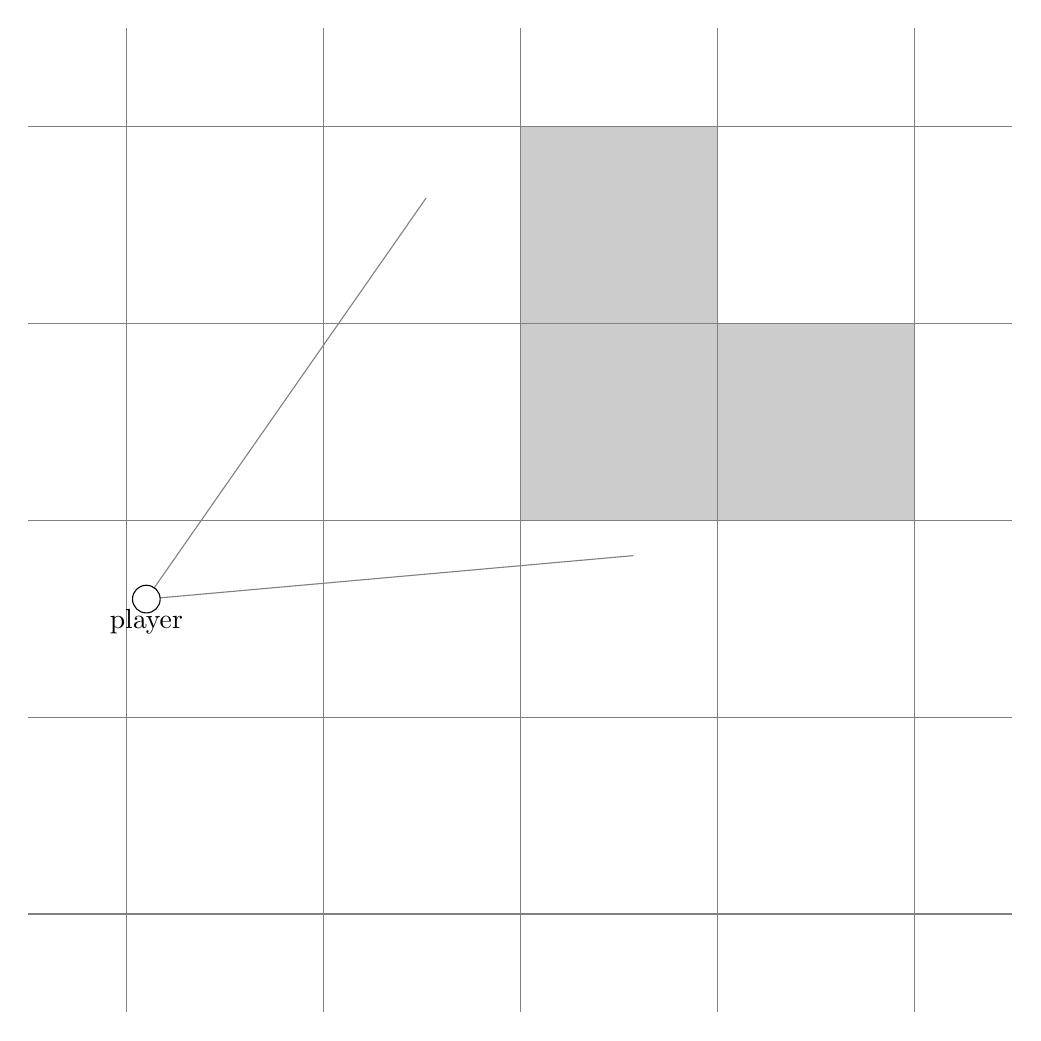
\begin{tikzpicture}[scale=2.5]


\coordinate(player) at (2.1,3.6) {};
\coordinate(intercept) at (4,5.2) {};






\fill[black!20!white, draw=black] (4,5) rectangle (5,6);
\fill[black!20!white, draw=black] (4,4) rectangle (5,5);
\fill[black!20!white, draw=black] (5,4) rectangle (6,5);

%grid
% vertical lines
\draw[draw=gray] (2,1.5) -- (2,6.5) ;
\draw[draw=gray] (3,1.5) -- (3,6.5) ;
\draw[draw=gray] (4,1.5) -- (4,6.5) ;
\draw[draw=gray] (5,1.5) -- (5,6.5) ;
\draw[draw=gray] (6,1.5) -- (6,6.5) ;

% horizontal lines
\draw[draw=gray] (1.5,2) -- (6.5,2) ;
\draw[draw=gray] (1.5,3) -- (6.5,3) ;
\draw[draw=gray] (1.5,4) -- (6.5,4) ;
\draw[draw=gray] (1.5,5) -- (6.5,5) ;
\draw[draw=gray] (1.5,6) -- (6.5,6) ;
%\draw[] 



\draw(player)node[below]{player};


\coordinate[](left_edge) at ($(player)!1!15:(intercept)$);
\coordinate[](right_edge) at ($(player)!1!325:(intercept)$);
\draw[draw=gray] (player) -> (left_edge) ;
\draw[draw=gray] (player) -> (right_edge) ;
\fill[draw=black, fill=white] (player) circle (2pt);



\end{tikzpicture}
\end{document}

\end{figure}

With a naive approach we could check for intersection at a regular interval. As the two rays draws below, it would works for some rays and fail for most of them.
\begin{figure}[H]
\centering
 \documentclass[tikz,border=2pt,png]{standalone}
\usepackage{tkz-euclide}
\begin{document}
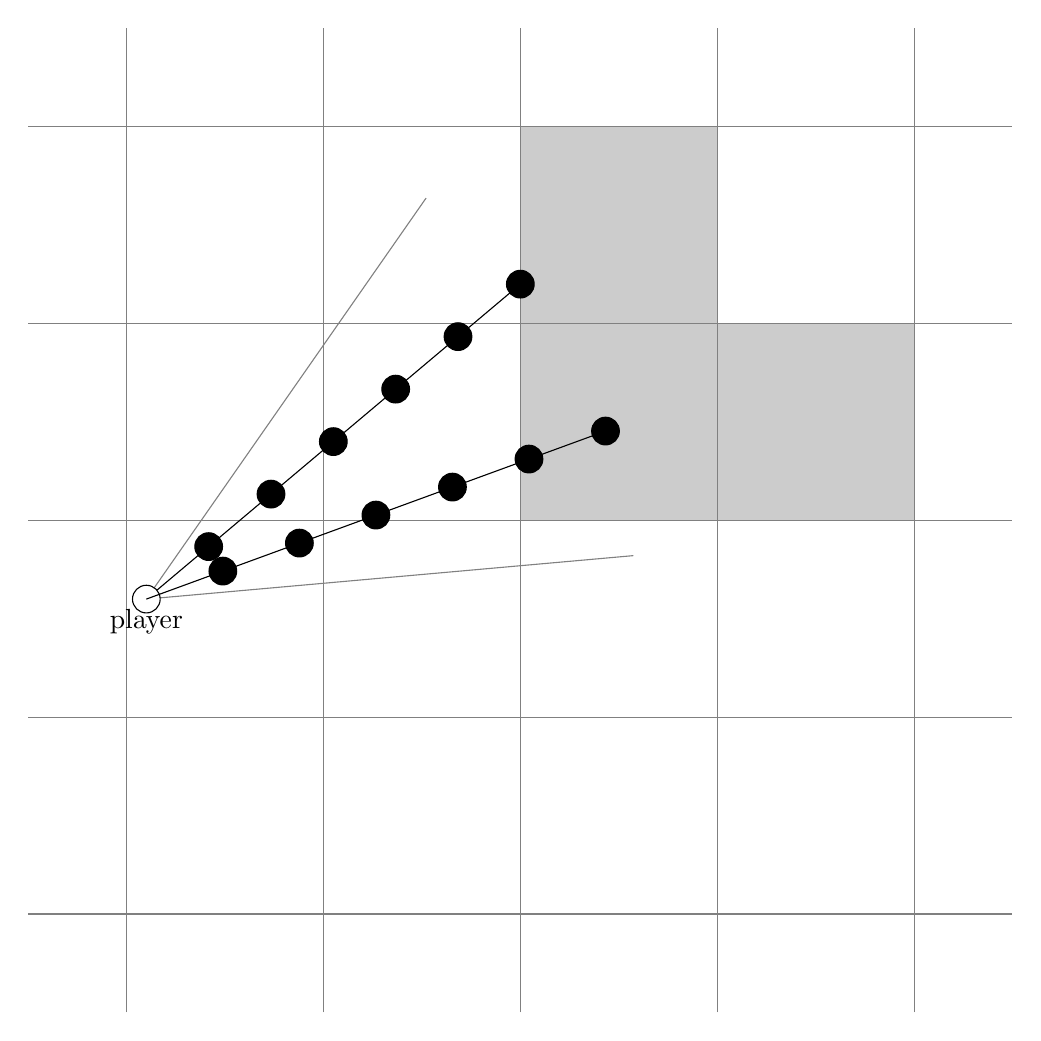
\begin{tikzpicture}[scale=2.5]


\coordinate(player) at (2.1,3.6) {};
\coordinate(intercept) at (4,5.2) {};

%FOV
\coordinate[](left_edge) at ($(player)!1!15:(intercept)$);
\coordinate[](right_edge) at ($(player)!1!325:(intercept)$);
\draw[draw=gray] (player) -> (left_edge) ;
\draw[draw=gray] (player) -> (right_edge) ;




\fill[black!20!white, draw=black] (4,5) rectangle (5,6);
\fill[black!20!white, draw=black] (4,4) rectangle (5,5);
\fill[black!20!white, draw=black] (5,4) rectangle (6,5);

%grid
% vertical lines
\draw[draw=gray] (2,1.5) -- (2,6.5) ;
\draw[draw=gray] (3,1.5) -- (3,6.5) ;
\draw[draw=gray] (4,1.5) -- (4,6.5) ;
\draw[draw=gray] (5,1.5) -- (5,6.5) ;
\draw[draw=gray] (6,1.5) -- (6,6.5) ;

% horizontal lines
\draw[draw=gray] (1.5,2) -- (6.5,2) ;
\draw[draw=gray] (1.5,3) -- (6.5,3) ;
\draw[draw=gray] (1.5,4) -- (6.5,4) ;
\draw[draw=gray] (1.5,5) -- (6.5,5) ;
\draw[draw=gray] (1.5,6) -- (6.5,6) ;
%\draw[] 

\draw[draw=black] (player) -- (intercept) ;
\fill[draw=black, fill=white] (player) circle (2pt);
\fill[draw=black] (intercept) circle (2pt);

\draw(player)node[below]{player};



\fill[draw=black] ( $ (player)!5/6!(intercept) $ ) circle (2pt);
\fill[draw=black] ( $ (player)!4/6!(intercept) $ ) circle (2pt);
\fill[draw=black] ( $ (player)!3/6!(intercept) $ ) circle (2pt);
\fill[draw=black] ( $ (player)!2/6!(intercept) $ ) circle (2pt);
\fill[draw=black] ( $ (player)!1/6!(intercept) $ ) circle (2pt);


\coordinate[](missed_intercept) at ($(player)!1!340:(intercept)$);
\draw[draw=black] (player) -- (missed_intercept) ;
\fill[draw=black] (missed_intercept) circle (2pt);
\fill[draw=black] ( $ (player)!5/6!(missed_intercept) $ ) circle (2pt);
\fill[draw=black] ( $ (player)!4/6!(missed_intercept) $ ) circle (2pt);
\fill[draw=black] ( $ (player)!3/6!(missed_intercept) $ ) circle (2pt);
\fill[draw=black] ( $ (player)!2/6!(missed_intercept) $ ) circle (2pt);
\fill[draw=black] ( $ (player)!1/6!(missed_intercept) $ ) circle (2pt);

\end{tikzpicture}
\end{document}

 \caption{blabla.}
\end{figure}

The solution for 100\% accuracy is to check for 'hit` when the ray cross the grid. This is why Wolfenstein 3D could only draw walls on a perpendicular grid.
\begin{figure}[H]
\centering
 \documentclass[tikz,border=2pt,png]{standalone}
\usepackage{tkz-euclide}
\begin{document}
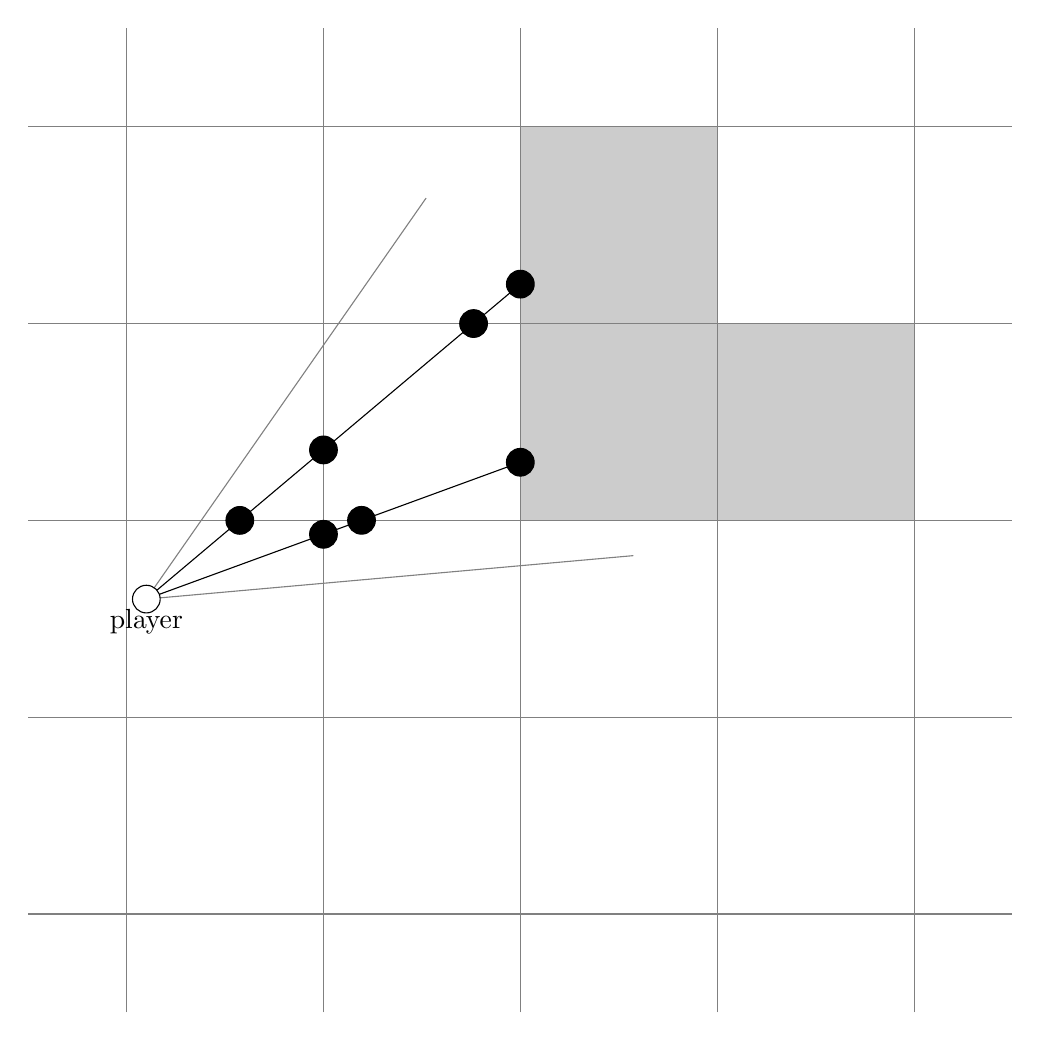
\begin{tikzpicture}[scale=2.5]


\coordinate(player) at (2.1,3.6) {};
\coordinate(intercept) at (4,5.2) {};






\fill[black!20!white, draw=black] (4,5) rectangle (5,6);
\fill[black!20!white, draw=black] (4,4) rectangle (5,5);
\fill[black!20!white, draw=black] (5,4) rectangle (6,5);

%grid
% vertical lines
\draw[draw=gray] (2,1.5) -- (2,6.5) ;
\draw[draw=gray] (3,1.5) -- (3,6.5) ;
\draw[draw=gray] (4,1.5) -- (4,6.5) ;
\draw[draw=gray] (5,1.5) -- (5,6.5) ;
\draw[draw=gray] (6,1.5) -- (6,6.5) ;

% horizontal lines
\draw[draw=gray] (1.5,2) -- (6.5,2) ;
\draw[draw=gray] (1.5,3) -- (6.5,3) ;
\draw[draw=gray] (1.5,4) -- (6.5,4) ;
\draw[draw=gray] (1.5,5) -- (6.5,5) ;
\draw[draw=gray] (1.5,6) -- (6.5,6) ;
%\draw[] 

%FOV
\coordinate[](left_edge) at ($(player)!1!15:(intercept)$);
\coordinate[](right_edge) at ($(player)!1!325:(intercept)$);
\draw[draw=gray] (player) -> (left_edge) ;
\draw[draw=gray] (player) -> (right_edge) ;

\draw[draw=black] (player) -- (intercept) ;

\fill[draw=black] (intercept) circle (2pt);

\draw(player)node[below]{player};

% check points for first intercept
\coordinate(line1_p1) at (0,4) {};
\coordinate(line1_p2) at (9,4) {};
\coordinate (check1) at (intersection of player--intercept and line1_p1--line1_p2);
\fill[draw=black] (check1) circle (2pt);

\coordinate(line2_p1) at (0,5) {};
\coordinate(line2_p2) at (9,5) {};
\coordinate (check2) at (intersection of player--intercept and line2_p1--line2_p2);
\fill[draw=black] (check2) circle (2pt);

%vertical intercelpt
\coordinate(line3_p1) at (3,0) {};
\coordinate(line3_p2) at (3,9) {};
\coordinate (check3) at (intersection of player--intercept and line3_p1--line3_p2);
\fill[draw=black] (check3) circle (2pt);



%intercept 2
\coordinate[](missed_intercept) at ($(player)!1!340:(intercept)$);


\coordinate(i2_line1_p1) at (0,4) {};
\coordinate(i2_line1_p2) at (9,4) {};
\coordinate (i2_check1) at (intersection of player--missed_intercept and i2_line1_p1--i2_line1_p2);
\fill[draw=black] (i2_check1) circle (2pt);

%vertical intercelpt
\coordinate(i2_line2_p1) at (4,0) {};
\coordinate(i2_line2_p2) at (4,9) {};
\coordinate (i2_check2) at (intersection of player--missed_intercept and i2_line2_p1--i2_line2_p2);
\fill[draw=black] (i2_check2) circle (2pt);


\coordinate(i2_line3_p1) at (3,0) {};
\coordinate(i2_line3_p2) at (3,9) {};
\coordinate (i2_check3) at (intersection of player--missed_intercept and i2_line3_p1--i2_line3_p2);
\fill[draw=black] (i2_check3) circle (2pt);
\draw[draw=black] (player) -- (i2_check2) ;

\fill[draw=black, fill=white] (player) circle (2pt);

\end{tikzpicture}
\end{document}

 \caption{blabla.}
\end{figure}
\par
DDA Algorythm:
 \par
\begin{figure}[H]
  \centering
 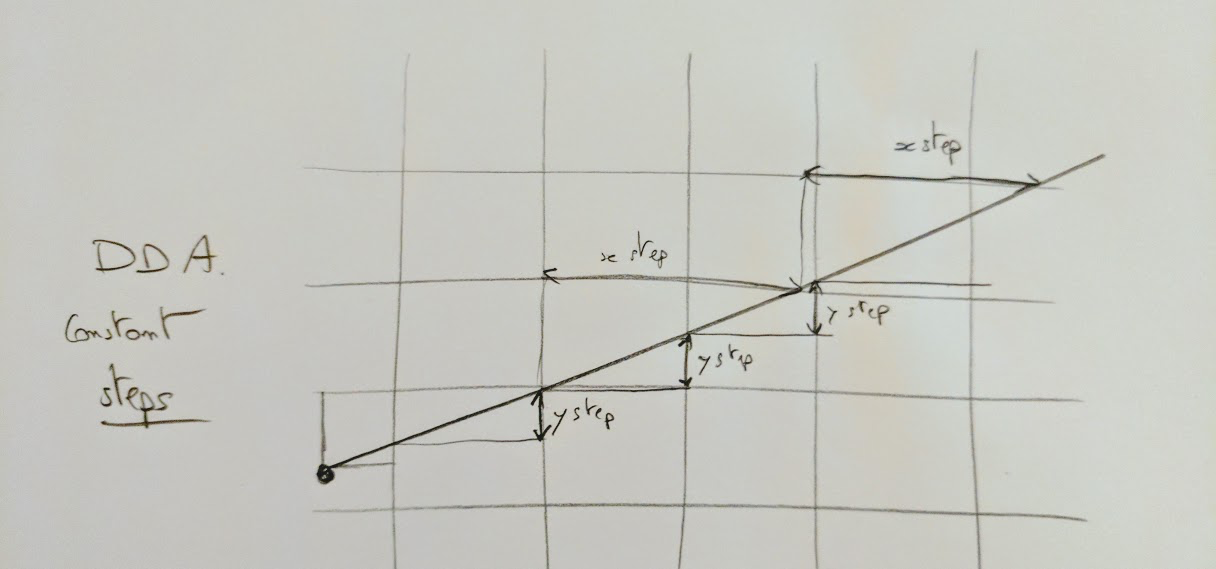
\includegraphics[width=\textwidth]{imgs/dda_explainer.png}
\end{figure}
\par

This way is fast. For the ray above, only four intersections checks had to done. For the one below only 3.\\
\par
And this explains why Wolfenstein3D maps are all flat, 64x64 grid aligned square blocks:\\
\par

\begin{figure}[H]
  \centering
 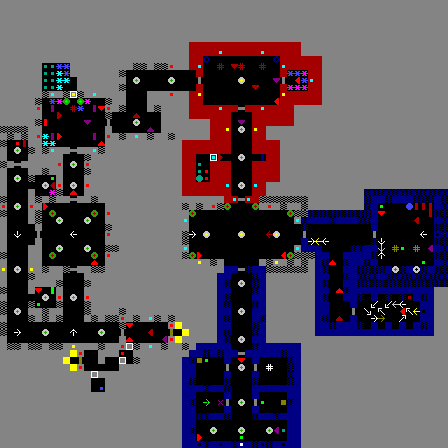
\includegraphics[width=\textwidth]{imgs/e1m1.png}
 \caption{The legendary E1M1. Player is the green arrow at the bottom.}
\end{figure}




\subsubsection{Call Apogee}
With map being simple and fast to draw, a contest was to be held: Find a special item in a particularly difficult to access place in the game and call the publisher (Apogee). The maze was located in Episode 2, Map 8:\\
\par
\begin{figure}[H]
  \centering
 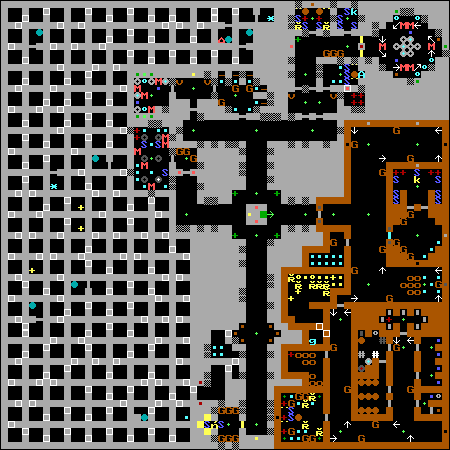
\includegraphics[width=\textwidth]{imgs/e2m8.png}
\end{figure}

\par
Behind a forest of push walls (white squares) and angry bosses (blue star), a sign finally showed up (the red triangle in the map above):\\
\par

\begin{figure}[H]
  \centering
 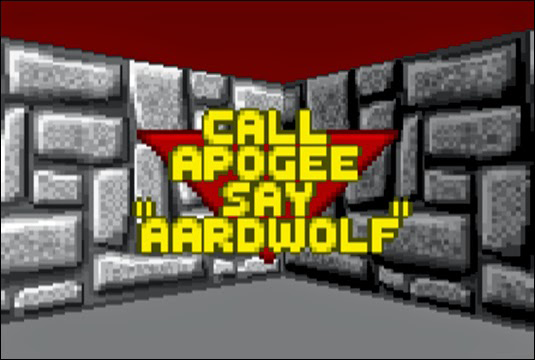
\includegraphics[width=\textwidth]{imgs/call_apogee.png}
\end{figure}
\par
However due to people reverse engineering the map format and cheat sites allowing players to find the maze, the sign was replaced with a squeleton with all game shipping during 1992
\par
\begin{fancyquotes}
"Call Apogee and say Aardwolf."  It's a sign that to this day is something
that I get asked about a lot.  This is a sign that appears on a wall in a
particularly nasty maze in Episode 2 Level 8 of Wolfenstein 3D.  The sign
was to be the goal in a contest Apogee was going to have, but almost
immediately after the game's release, a large amount of cheat and mapping
programs were released.  With these programs running around, we felt that
it would have been unfair to have the contest and award a prize.  The sign
was still left in the game, but in hindsight, probably should have been
taken out.  To this day, Apogee gets letters and phone calls and asking
what Aardwolf is, frequently with the question, "Has anyone seen this yet?"\\
\\
Also, in a somewhat related issue, letters were shown after the highest score
in the score table in some revisions of the game.  These letters were to be
part of another contest that got scrapped before it got started, where we were
going to have people call in with their scores and tell us the code; we'd then
be able to verify their score.  However, with the cheat programs out there,
this got scrapped too.\\
\\
Basically, "Aardwolf" and the letters mean nothing now.  Also note that if
you found the Aardwolf sign in the game (without cheating), there's a VERY
strong chance that you're stuck in there.  The only way out may be to restart,
or load a saved game from before you went into that maze.\\
\\
\textbf{Joe Siegler - Past Pioneers of the Shareware Revolution}
\end{fancyquotes}














 
 
 
 
 
 
 
 
\subsubsection{Raycasting: DDA Algorithm}
The raycasting algorithm is calld DDA\footnote{Digital Differential Analysis, commonly used in CG world to draw a line.}. It is a fully handcrafted 740 lines of assembly routine name \cw{PROC AsmRefresh}. Represented in C for readability it consists of two while looks (one checking vertical intersection and one checking the horizontal) ping-ponging with each other via goto. It is highyt unorthodox and super efficient:\\
\par

\begin{minipage}{\textwidth}
\lstinputlisting[language=C]{code/flipflop.c}
\end{minipage}

\note{Trivia:} To accelerate \cw{cos} and \cw{sin} calculation, the engine uses lookup table: One entry for each 360 degres.




\begin{fancyquotes}
Why a raycaster instead of a rasterizer?\\
\par
Much was made about the "ray casting" used in Wolfenstein, but the real reason for it was that I had a lot of trouble with wall-span rendering in Catacombs 3D.  C3D (and Hovertank before that) shipped with various graphics glitches that you could get in some combinations of map block configurations, position, and viewing angle.  Some were due to fixed point precision issues not being handled optimally, and some were due to clipping and culling issues that I didn't really get a handle on until a couple years later.  In any case, they bothered me a lot.  Spurious graphics glitches do a lot of harm to the sense of immersion in a game, and I very much wanted Id games to feel "rock solid".
 \bigskip \\
There was a clear performance cost to it - doing 320 traces through a tile map and treating each column independently is much slower than looping through a few long wall segments.  However, the resulting code was small and very regular compared to the hairball of my wall span renderers, and it did deliver the rock-solid feel I wanted.
 \bigskip \\
If you made extremely jagged block maps that would turn into many dozen independent wall segments, the ray casting could start to look like a good performance choice, but few scenes were even close to that.  This is exactly the same ray tracing versus rasterization performance tradeoff that is still being made today, but now it is "how many tens of millions of triangles per frame to ray tracing break-even" instead of "how many dozen wall segments".
 \bigskip \\
\textbf{John Carmack - Programmer}
 \end{fancyquotes}











\subsubsection{FishEye}
With a fast way to find the intersection between a ray and the walls, the distance is calculated in \cw{CalcHeight}:\\

\begin{minipage}{\textwidth}
\lstinputlisting[language=C]{code/CalcHeight.c}
\end{minipage}

The code is not what one would expect: The raycasting algorithm is supposed to cast a ray for each pixel column and use the distance \codeword{d} to infer the column's heigh on screen. So one would have expected to see a formula like:
$ d = \sqrt{dx^2 + dy^2}$ . But instead it looks like: $d = dx * \cos(\alpha) - dy * \sin(\alpha) $! Something is fishy here ;) !\\
\par
\begin{figure}[H]
\centering
 %\documentclass[tikz,border=2pt,png]{standalone}
%\usepackage{tkz-euclide}
%\usetkzobj{all}
%\begin{document}
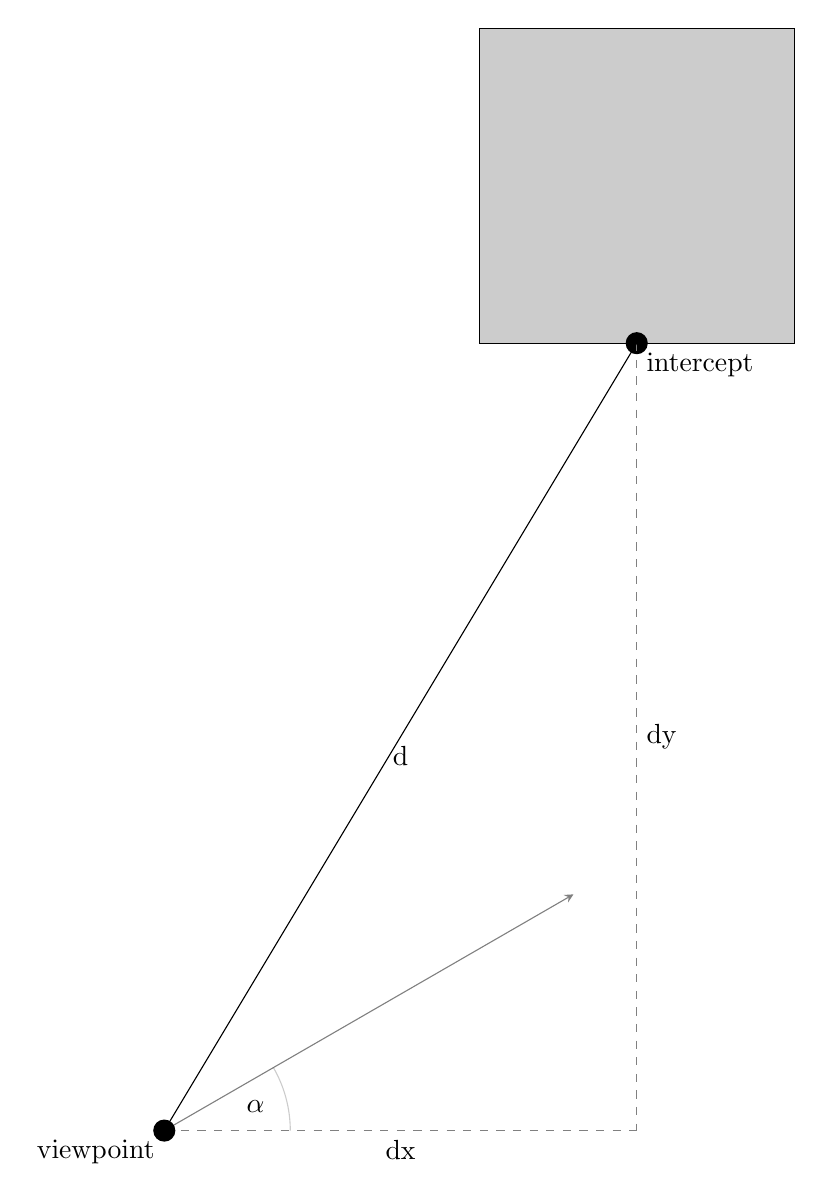
\begin{tikzpicture}[scale=2.0]

\coordinate(origin) at (0,0)[label=below:view] {};
\coordinate(yaxis) at (0,6.5){};
\coordinate(xaxis) at (6,0) {};
\coordinate(angle) at (30:3);
\coordinate(intercept) at (3,5) {};

\node[below left] (orign) {viewpoint};
\node[below right] (_XX) at (intercept) {intercept};

% AXIS
%\draw[->,draw=black,>=stealth] (origin)  -- (xaxis) ;
%\draw[->,draw=black,>=stealth] (origin)  -- (yaxis) ;
%\draw[draw=black] (origin)  -- (0,-0.5) ;
%\draw[draw=black] (origin)  -- (-0.5,0) ;

% WALL
\fill[black!20!white, draw=black] (2,5) rectangle (4,7);
%\fill[black!20!white, draw=black] (4,5) rectangle (6,7);
%\fill[black!20!white, draw=black] (4,3) rectangle (6,5);


\fill (intercept) circle (2pt);


\draw[->,draw=gray,>=stealth] (origin)  -- (angle) ;

\coordinate (dx) at ($(origin)!(intercept)!(xaxis)$);
\draw[draw=gray,>=stealth,dashed] (origin) -- node[below] {dx} (dx);
\draw[draw=gray,>=stealth,dashed] (intercept) -- node[right] {dy}(dx);

\tkzMarkAngle[fill= gray,size=0.8cm,opacity=.2](xaxis,origin,angle)
\tkzLabelAngle[pos = 0.6](xaxis,origin,angle){$\alpha$}

\fill[fill=black] (origin) circle (2pt);

\draw[] (origin) -- node[below] {d} ++(intercept) ;

%\draw[] 


\end{tikzpicture}
%\end{document}
 \caption{Raycasting using distance d} \label{fig:Raycasting2}
\end{figure}

In this drawing the player is located at viewpoint with a view angle \begin{math}\alpha\end{math}. The distance \codeword{d} is a straight line between the player point of view and the location where the ray hit the line which can be obtained with $d = \sqrt{dx^2 + dy^2}$. Such an algorithm would result in a "fisheye effect". It is not very noticeable when a wall is far:

\begin{figure}[H]
\centering
 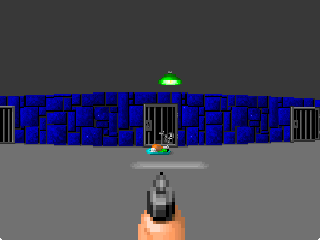
\includegraphics[width=\textwidth]{imgs/fish_eye/bad_mild.png}
 \caption{Fish eye effect: Mild}. \label{fig:mips}
 \end{figure}

But it gets worse when you get closer:
\begin{figure}[H]
\centering
 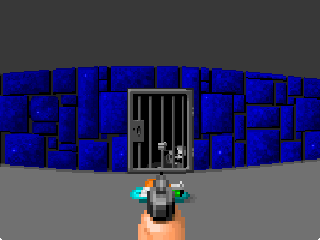
\includegraphics[width=\textwidth]{imgs/fish_eye/bad_ok.png}
 \caption{Fish eye effect: Bad} \label{fig:mips}
 \end{figure}

And become unbearable when very close:
 \begin{figure}[H]
\centering
 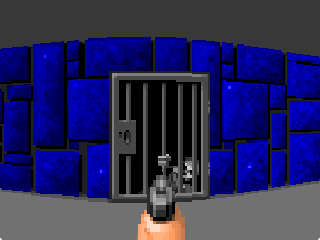
\includegraphics[width=\textwidth]{imgs/fish_eye/bad_bad.png}
 \caption{Fish eye effect: AAAAARG} \label{fig:mips}
 \end{figure}
 
To avoid this distortion and get a more pleasant rendition, what must be used is not the direct distance d but d projected on the perpendicular of the view direction (z):

\begin{figure}[H]
\centering
 %\documentclass[tikz,border=2pt,png]{standalone}
%\usepackage{tkz-euclide}
%\usetkzobj{all}
%\begin{document}
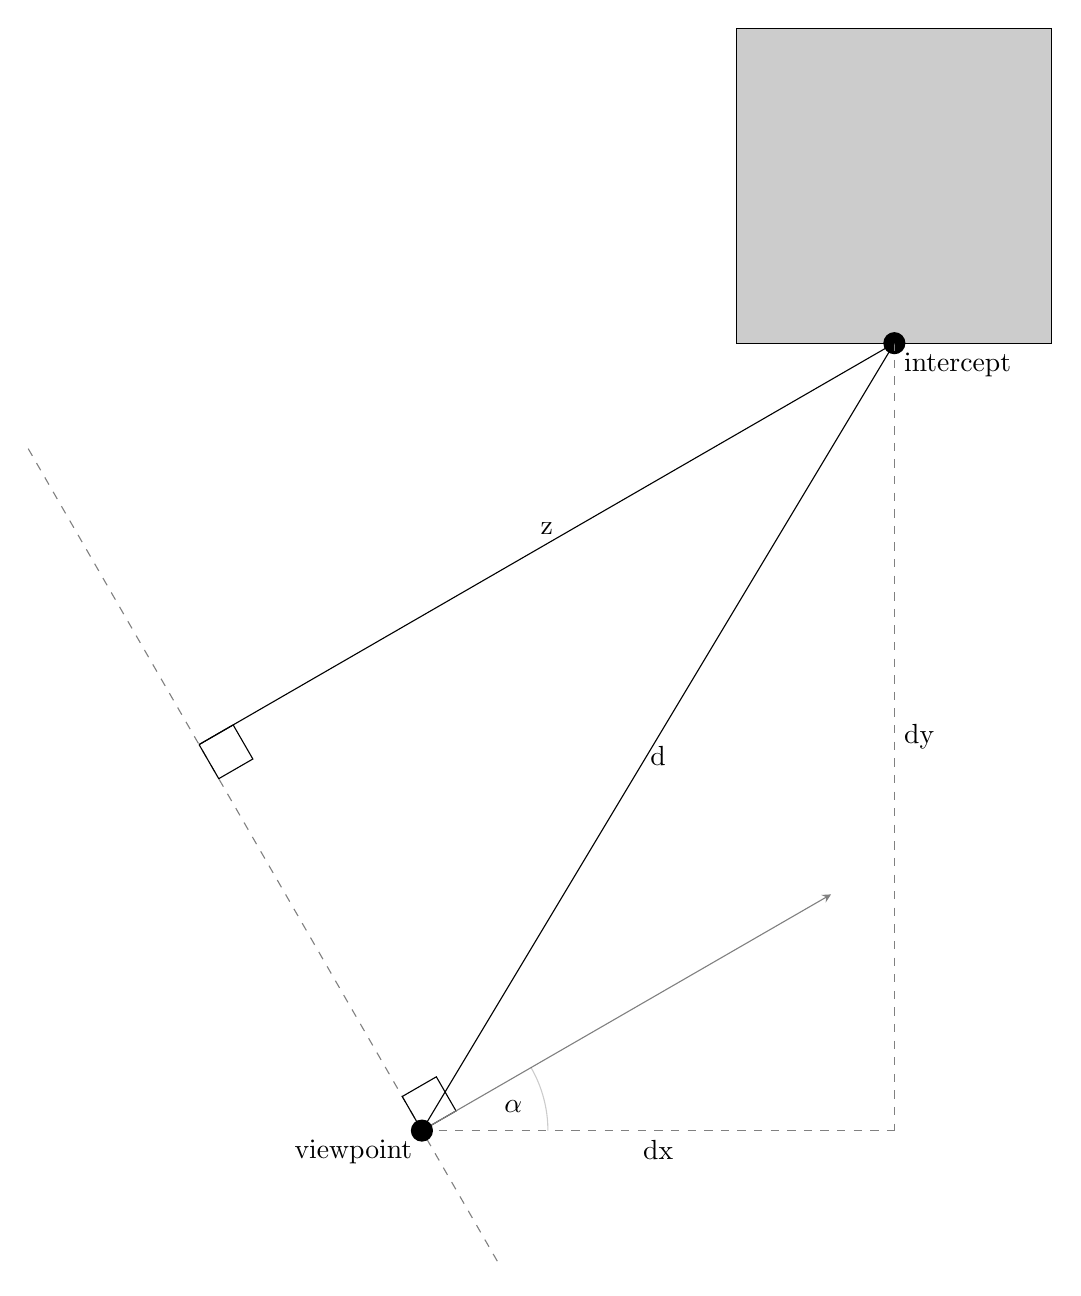
\begin{tikzpicture}[scale=2.0]

\coordinate(origin) at (0,0)[label=below:view] {};
\coordinate(yaxis) at (0,6.5){};
\coordinate(xaxis) at (6,0) {};
\coordinate(angle) at (30:3);
\coordinate(intercept) at (3,5) {};

\node[below left] (orign) {viewpoint};
\node[below right] (_XX) at (intercept) {intercept};

% plan
\coordinate(planA) at (120:5);
\coordinate(planB) at (-60:1);
\draw[draw=gray,dashed] (planA) -- (planB);
% AXIS
%\draw[->,draw=black,>=stealth] (origin)  -- (xaxis) ;
%\draw[->,draw=black,>=stealth] (origin)  -- (yaxis) ;
%\draw[draw=black] (origin)  -- (0,-0.5) ;
%\draw[draw=black] (origin)  -- (-0.5,0) ;

% WALL
\fill[black!20!white, draw=black] (2,5) rectangle (4,7);
%\fill[black!20!white, draw=black] (4,5) rectangle (6,7);
%\fill[black!20!white, draw=black] (4,3) rectangle (6,5);

% projected intercept
\coordinate (proj_intercept) at ($(planA)!(intercept)!(planB)$);
\draw[draw=black] (proj_intercept) -- node[above] {z} (intercept);

\tkzMarkRightAngle(intercept,proj_intercept,origin);
\tkzMarkRightAngle(angle,origin,proj_intercept);

\fill (intercept) circle (2pt);

% Angle
\draw[->,draw=gray,>=stealth] (origin)  -- (angle) ;

\coordinate (dx) at ($(origin)!(intercept)!(xaxis)$);
% DX and DY
\draw[draw=gray,>=stealth,dashed] (origin) -- node[below] {dx} (dx);
\draw[draw=gray,>=stealth,dashed] (intercept) -- node[right] {dy}(dx);

\tkzMarkAngle[fill= gray,size=0.8cm,opacity=.2](xaxis,origin,angle)
\tkzLabelAngle[pos = 0.6](xaxis,origin,angle){$\alpha$}

\fill[fill=black] (origin) circle (2pt);

% D libe
\draw[] (origin) -- node[below] {d} ++(intercept) ;

%\draw[] 


\end{tikzpicture}
%\end{document}
 \caption{blabla.} \label{fig:Raycasting2}
\end{figure}

This projection (z) is mathematically hard to calculate in one go (especially with fixed point). The trick is to break it down in two components and use your highschool mnemonic: SOH-CAH-TOA!\\

\begin{figure}[H]
\centering
 %\documentclass[tikz,border=2pt,png]{standalone}
%\usepackage{tkz-euclide}
%\usetkzobj{all}
%\begin{document}
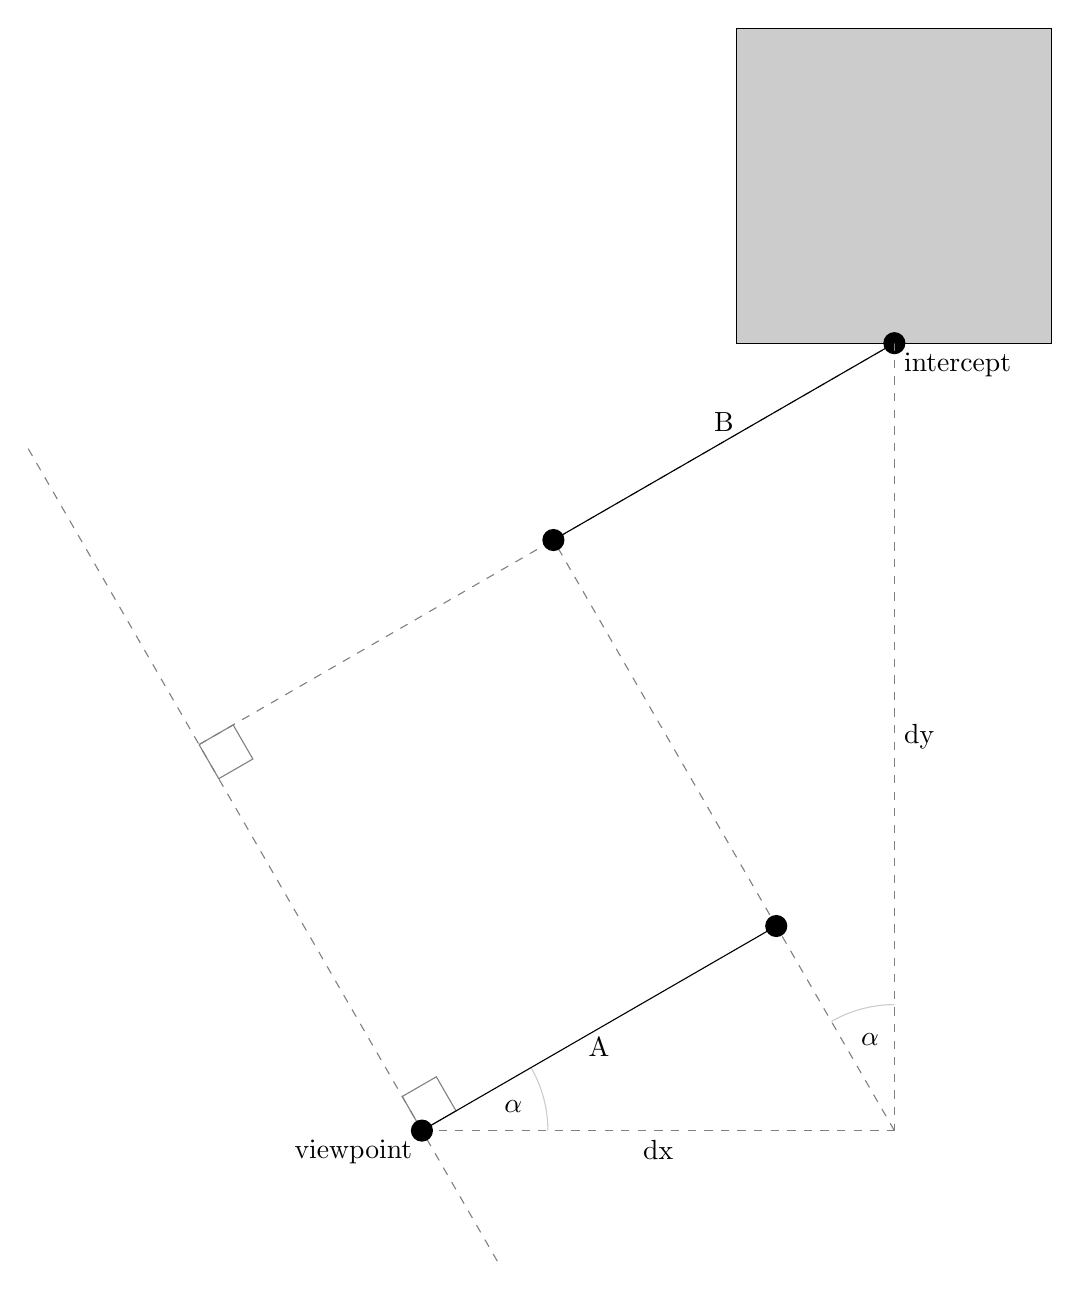
\begin{tikzpicture}[scale=2.0]

\coordinate(origin) at (0,0)[label=below:view] {};
\coordinate(yaxis) at (0,6.5){};
\coordinate(xaxis) at (6,0) {};
\coordinate(angle) at (30:3);
\coordinate(intercept) at (3,5) {};

\node[below left] (orign) {viewpoint};
\node[below right] (_XX) at (intercept) {intercept};

% plan
\coordinate(planA) at (120:5);
\coordinate(planB) at (-60:1);
\draw[draw=gray,dashed] (planA) -- (planB);
% AXIS
%\draw[->,draw=black,>=stealth] (origin)  -- (xaxis) ;
%\draw[->,draw=black,>=stealth] (origin)  -- (yaxis) ;
%\draw[draw=black] (origin)  -- (0,-0.5) ;
%\draw[draw=black] (origin)  -- (-0.5,0) ;

% WALL
\fill[black!20!white, draw=black] (2,5) rectangle (4,7);
%\fill[black!20!white, draw=black] (4,5) rectangle (6,7);
%\fill[black!20!white, draw=black] (4,3) rectangle (6,5);

% projected intercept
\coordinate (proj_intercept) at ($(planA)!(intercept)!(planB)$);
\draw[draw=gray,dashed] (proj_intercept) -- node[above] {} (intercept);

\tkzMarkRightAngle[draw=gray](intercept,proj_intercept,origin);
\tkzMarkRightAngle[draw=gray](angle,origin,proj_intercept);

\fill (intercept) circle (2pt);

% Angle
%\draw[->,draw=gray,>=stealth] (origin)  -- (angle) ;

\coordinate (dx) at ($(origin)!(intercept)!(xaxis)$);
% DX and DY
\draw[draw=gray,>=stealth,dashed] (origin) -- node[below] {dx} (dx);
\draw[draw=gray,>=stealth,dashed] (intercept) -- node[right] {dy}(dx);

\tkzMarkAngle[fill= gray,size=0.8cm,opacity=.2](xaxis,origin,angle)
\tkzLabelAngle[pos = 0.6](xaxis,origin,angle){$\alpha$}

\fill[fill=black] (origin) circle (2pt);

\coordinate (A) at ($(origin)!(dx)!(angle)$);
\draw[] (origin)  -- node[below] {A} (A) ;

\coordinate (B) at ($(proj_intercept)!(dx)!(intercept)$);
\draw[] (intercept)  -- node[above] {B} (B) ;

\draw[draw=gray,dashed] (dx) -- (B) ;

\fill (A) circle (2pt);
\fill (B) circle (2pt);

\tkzMarkAngle[fill= gray,size=0.8cm,opacity=.2](intercept,dx,A)
\tkzLabelAngle[pos = 0.6](intercept,dx,A){$\alpha$}

\end{tikzpicture}
%\end{document}
 \caption{A combination of SOH A=($dx * \cos(\alpha)$) and CAH B=($ dy * \sin(\alpha) $) gives $d = dx * \cos(\alpha) - dy * \sin(\alpha) $ gives the expected result.}
\end{figure}

 Which is enough to give pleasant straigh lines. Following a wall uncorrected and the same location with projected distance:\\
 \begin{figure}[H]
\centering
 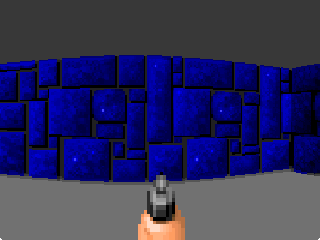
\includegraphics[width=\textwidth]{imgs/fish_eye/fish_eye.png}
  \caption{Fish eye: Uncorrected} 
 \end{figure}
 

  \begin{figure}[H]
\centering
 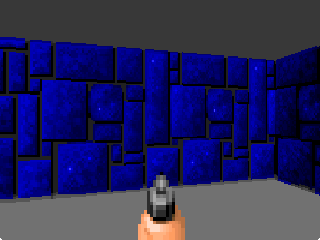
\includegraphics[width=\textwidth]{imgs/fish_eye/fish_eye_corrected.png}
\caption{Fish eye: Corrected} 
 \end{figure}
 \par
 An other example with the starting screen:\\
 \par
  \begin{figure}[H]
\centering
 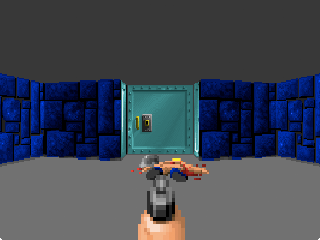
\includegraphics[width=\textwidth]{imgs/fish_eye/fish_eyed_start_screen2.png}
  \caption{Fish eye: Uncorrected} 
 \end{figure}
 \par

  \begin{figure}[H]
\centering
 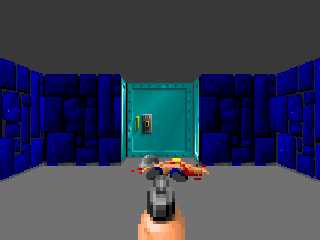
\includegraphics[width=\textwidth]{screenshots/wolf3d_7_fullframe.png}
  \caption{Fish eye: Corrected} 
 \end{figure}
 \par
 Note: Why substract values insted of adding them ? The coordinate system has its origin at the upper left which inverse the sin value. To compensate for it, the correction math uses substraction instead of addition.













\subsection{Drawing walls}
Drawing the wall may sound easy. After how complicated can it be to scale a 64 pixels tall texture on the screen, centered vertically? It turns out if you want to do it fast you can apply a few optimization. This part is where lies the two secrets of the engine speed: Compiled scalers and defered column rendering.\\
\par


\subsubsection{Compiled scalers}
With a distance available for a column, the engine is able to calculate a height for that column. All columns of pixels representing the walls are centered vertically and either magnified or minified:\\
\par
 \begin{figure}[H]
\centering
 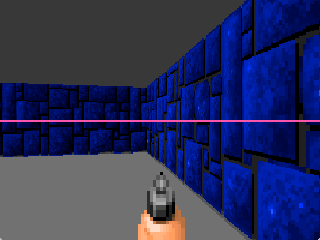
\includegraphics[width=\textwidth]{imgs/scaler_valign.png}
 \end{figure}
\par

The naive approach would be to use a generic routine:\\
\begin{verbatim}
void drawRoutine(int height, void* src, void* dst) {
  
}
\end{verbatim}
\par
But that would be a lot of instruction for sometimes only a few pixels generated. There is a faster way: Generate code specialized to drawing all height of wall from 1 pixels to 200 (the height of the screen).\\
\par
 \begin{figure}[H]
\centering
 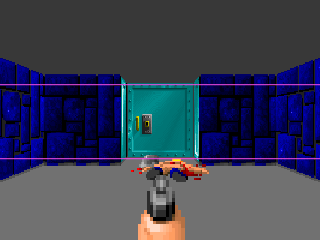
\includegraphics[width=\textwidth]{imgs/scaling_walls.png}
 \end{figure}
\par
Everything not between the pink lines (64 pixels tall) is either minified or magnified. It is a significant task to perform at runtime, involving fraction (of course done via fixed point arithmetics). To speed up this phase, the engine generate executable x86 code when the screen size is set (at startup or upon user choices).
TODO: Show a lower resolution photo.\\
TODO: Show precompiled scaler ram consumption.\\
Every column of pixels are centered vertically.



TODO: Pseudo-code here\\
\par
Builds a compiled scaler object that will scale a 64 tall object to the given height (centered vertically on the screen).
\codeword{SetupScaling}\\
\codeword{BuildCompScale}
Trivia: What as the memory budget of the scaller? JC had to cut corners. What was the cost before cutting corners.\\
\par
\begin{minipage}{\textwidth}
\lstinputlisting[language=C]{code/compscale.c}
\end{minipage}













\subsubsection{Defered drawing:}
A naive implementation of the raycaster would be:\\

\begin{minipage}{\textwidth}
\lstinputlisting[language=C]{code/naive_raycaster_pseudocode.c}
\end{minipage}
\par
But the engine is different: It buffers what to draw:\\
\par
\begin{minipage}{\textwidth}
\lstinputlisting[language=C]{code/wolf3d_raycaster_pseudocode.c}
\end{minipage}

Rendition is deferred because the engine allows itself to cheat a little: If a ray is cast and hits the same block and in the same
texture column, the two rays are considered similar. If two rays are similar they are drawn at the same height. The visual result is 
barely noticable. But this cheat allows to draw up to eight column of pixel in three write operations (in practice it is more like two columns
with one write operation). The details of this are in the method \codeword{ScalePost} in \codeword{WL\_DRAW.C}.\\

Note: A \quotes{post} is a column of pixel belonging to a wall.\\
ScalePost is written in assembly and performs a maximum of three pass to draw a maximum of eight columns of pixels.\\
\par 
\begin{minipage}{\textwidth}
\lstinputlisting[language=C]{code/ScalePost.c}
\end{minipage}
Because there can be many combinations of VGA bank alignment and number of pixels to draw:

\begin{figure}[H]
\centering
 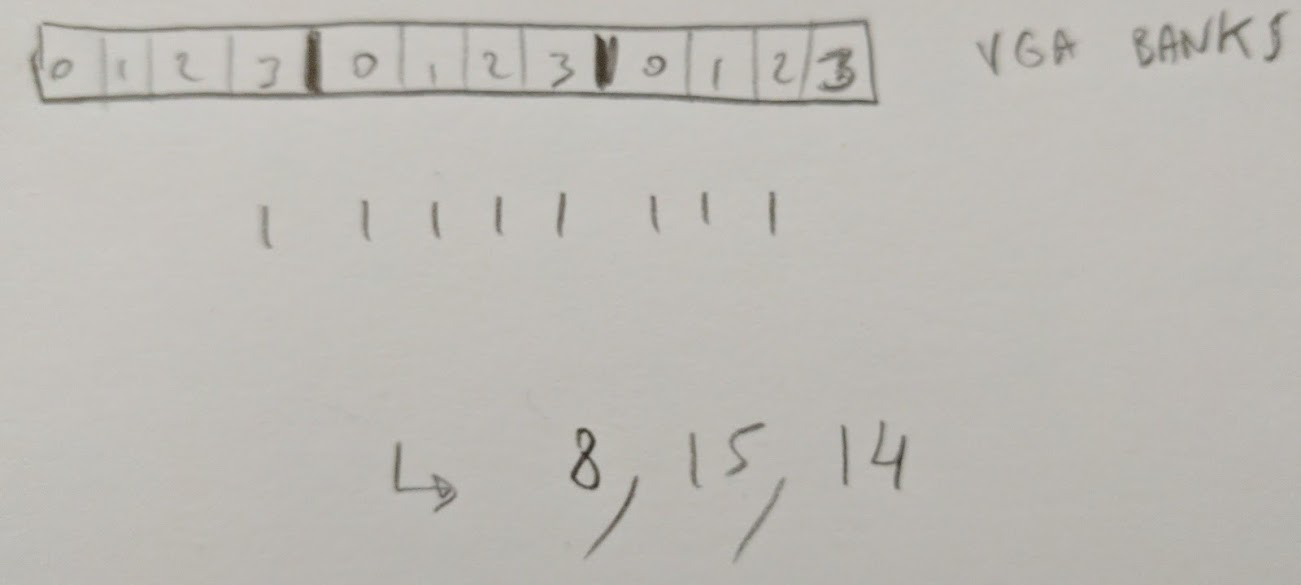
\includegraphics[width=\textwidth]{imgs/scalePost_explanation1.png}
 \end{figure}
 
 \begin{figure}[H]
 \centering
 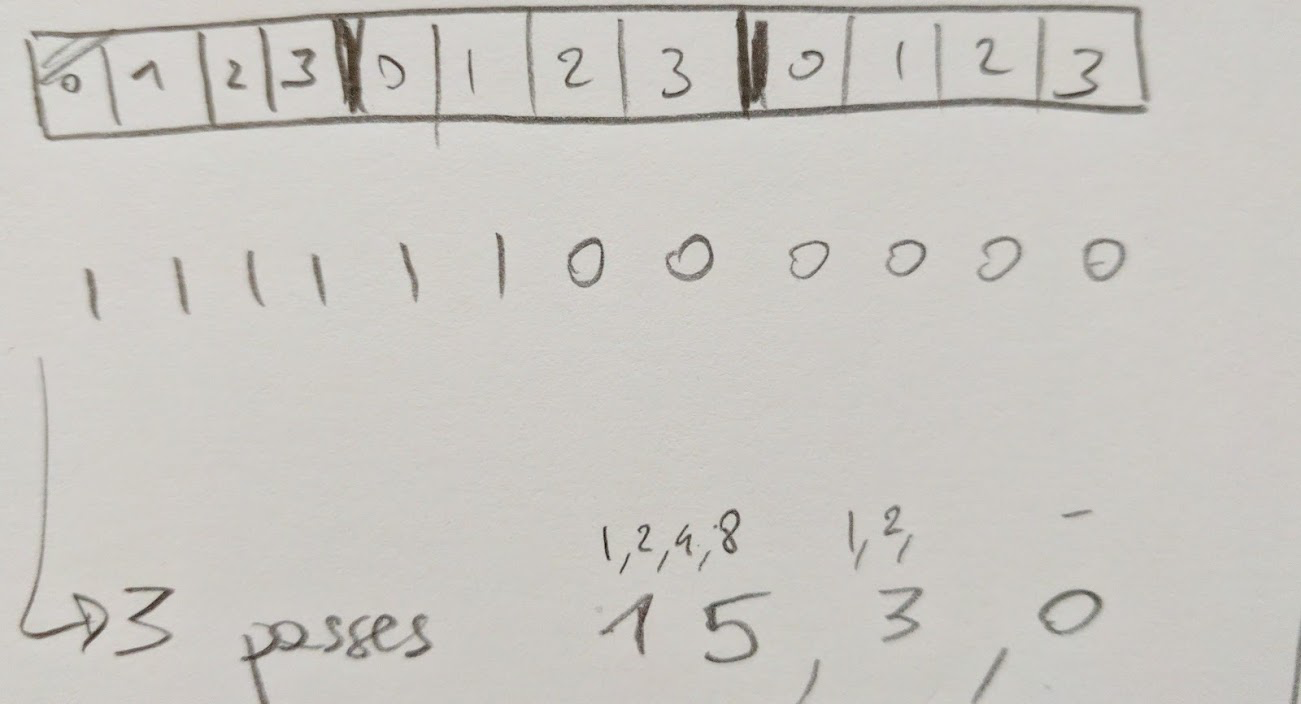
\includegraphics[width=\textwidth]{imgs/scalePost_explanation2.png}
 \end{figure}
The instruction \codeword{or al , al} can be surprising. It means test if al is equal to zero and set the flag. Back in the day it was more populate than \codeword{test al, al}
 the VGA bank masks are harcoded in an array: One for each pass:\\
 \par
 \begin{minipage}{\textwidth}
\lstinputlisting[language=C]{code/hardcoded_masks.c}
\end{minipage}
TODO: Were images stored rotated 90degres to increase cache hit ? No way, this was aimed at 386. BUT that would make the drawing easier !!

In the following example, the left wall is magnified. several rays hit the wall at the same texture location.
\begin{figure}[H]
 \centering
 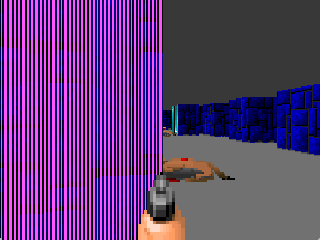
\includegraphics[width=\textwidth]{imgs/post_optimization_1_pink_show.png}
\end{figure}
The engine takes advantage of it and draw several columns (posts) efficiently with the VGA. The engine was altered to show the optimized posts in pink.
\begin{figure}[H]
 \centering
 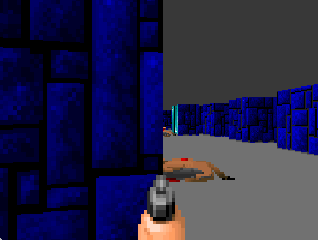
\includegraphics[width=\textwidth]{imgs/post_optimization_1_show.png}
\end{figure}

In the previous scene, 20\% of the wall was optimized away. In the next two screenshot, the same process, this time with the `eagle' texture:
\begin{figure}[H]
 \centering
 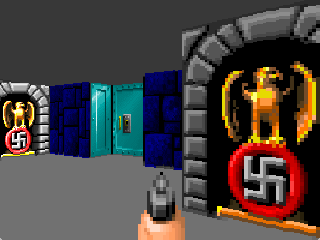
\includegraphics[width=\textwidth]{imgs/post_optimization_2_show.png}
\end{figure}


\begin{figure}[H]
 \centering
 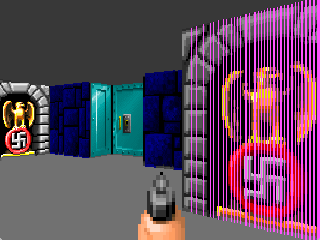
\includegraphics[width=\textwidth]{imgs/post_optimization_2_pink_show.png}
\end{figure}
 
To draw several column of pixels at the same time, the engine exploit the VGA banks and the masking mechanism seen in the Hardware section.
Since up to eight column can be similar, there are many case of figure depending on the aligment with the VGA banks and how many pixels to draw:

Example























\subsubsection{Texturing}


Pre-Lighted texture.\\

  \begin{figure}[H]
\centering
 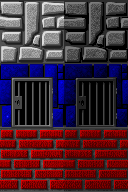
\includegraphics[width=\textwidth]{imgs/baked_lights.png}
 \caption{3D Rendere Phase 1: Backed lights} \label{fig:backee_lights}
 \end{figure}





 





\subsubsection{Door}
Doors have no tickness.\\
doorposition[] holds the amount the door is open, ranging from 0 to 0xffff
  this is directly accessed by AsmRefresh during rendering\\
  // don't close on anything solid\\
\begin{figure}[H]
 \centering
 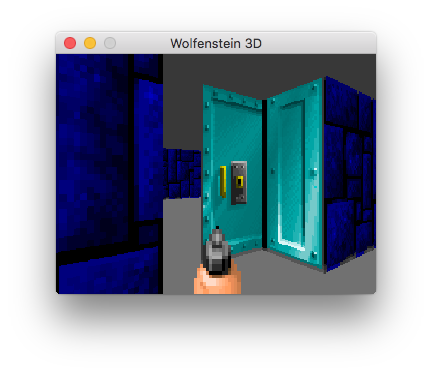
\includegraphics[width=\textwidth]{imgs/door_flat.png}
\end{figure}

\par
TODO: Explaih half step added.\\
\par 
 \par
\begin{figure}[H]
  \centering
 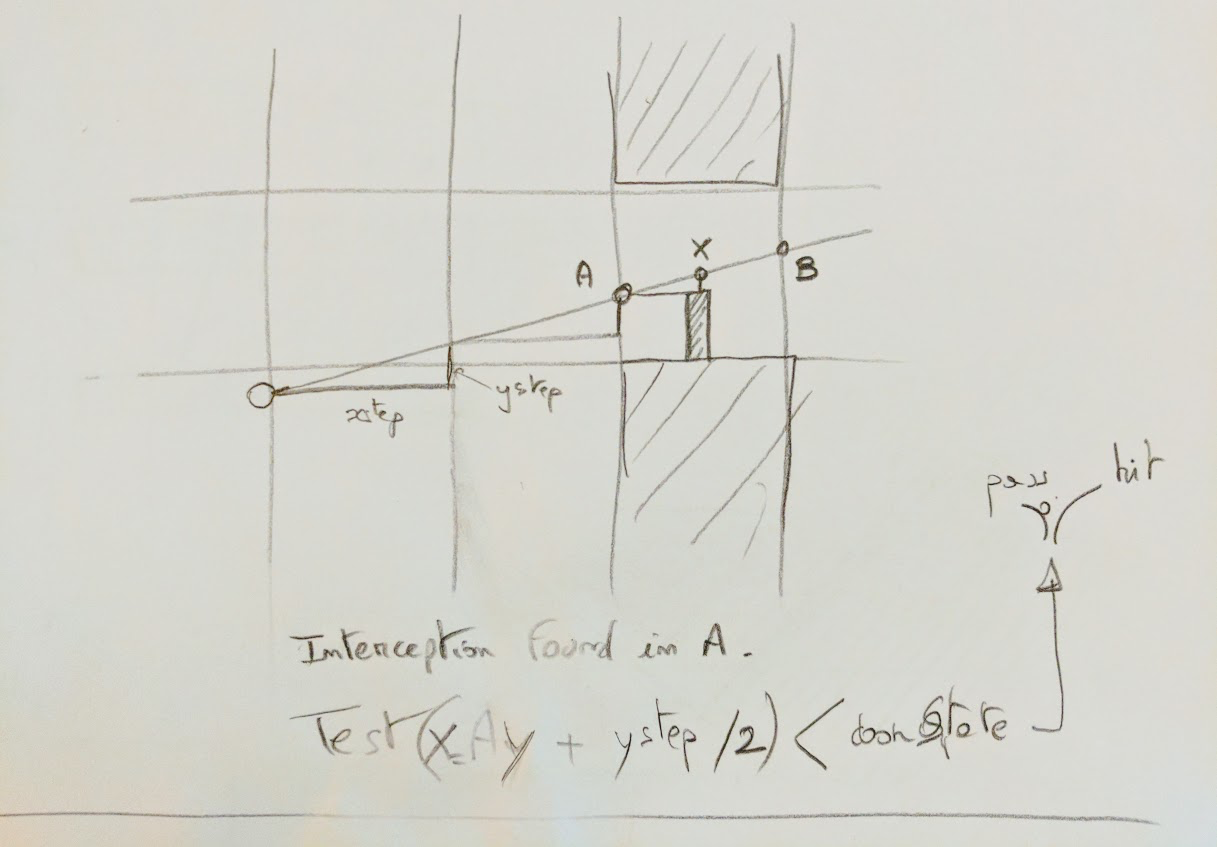
\includegraphics[width=\textwidth]{imgs/test_door.png}
\end{figure}
\par












\subsubsection{Push walls} 
Push walls are very similar to doors except they "open" away from the player instead of sideway.


















\subsection{Drawing things}
To determine what is visible and draw things properly is hard. Michael Abrash summarized the domain of the problem well:\\

\begin{fancyquotes}
I want to talk about what is, in my book, the toughest 3-D problem of all, visible surface determination (drawing the proper surface at each pixel), and its close relative, culling (discarding non-visible polygons as quickly as possible, a way of accelerating visible surface determination). In the interests of brevity, I’ll use the abbreviation VSD to mean both visible surface determination and culling from now on.
 \bigskip \\
Why do I think VSD is the toughest 3-D challenge? Although rasterization issues such as texture mapping are fascinating and important, they are tasks of relatively finite scope, and are being moved into hardware as 3-D accelerators appear; also, they only scale with increases in screen resolution, which are relatively modest.
 \bigskip \\
In contrast, VSD is an open-ended problem, and there are dozens of approaches currently in use. Even more significantly, the performance of VSD, done in an unsophisticated fashion, scales directly with scene complexity, which tends to increase as a square or cube function, so this very rapidly becomes the limiting factor in doing realistic worlds. I expect VSD increasingly to be the dominant issue in realtime PC 3-D over the next few years, as 3-D worlds become increasingly detailed.
 \bigskip \\
\bigskip \\
\textbf{Michael Abrash - Programmer}
 \end{fancyquotes}
 
 Wolf3D uses two mechanism to make sure things are draw properly:
 \begin{enumerate}
  \item While casting each ray, memorize which cells were visited by the ray. This is used to know which "things" to draw.
  \item Upon drawing a wall column, save the height of that wall. This is done to clip "things" to draw.
 \end{enumerate}
 


 At the beginning of each 3D rendition, the engine clears the:
 \lstinputlisting[language=C]{code/clear_vis_wold3d.c}
 Note that because register are 2 bytes wide, an array of 64x64=4096 bytes can be zeroed in 2048 iterations. Nowadays it is more efficient to use the C library.
 \lstinputlisting[language=C]{code/clear_vis_modern.c}
 Later in the assembly hand crafted procedure \codeword{AsmRefresh} we can find where this array is populated:
  \lstinputlisting[language={[x86masm]Assembler}]{code/mark_vis_wold3d.asm}
  If we take the example of the starting screen, we can see which tile were marked at visible:
  
  
\begin{figure}[H]
  \centering
  
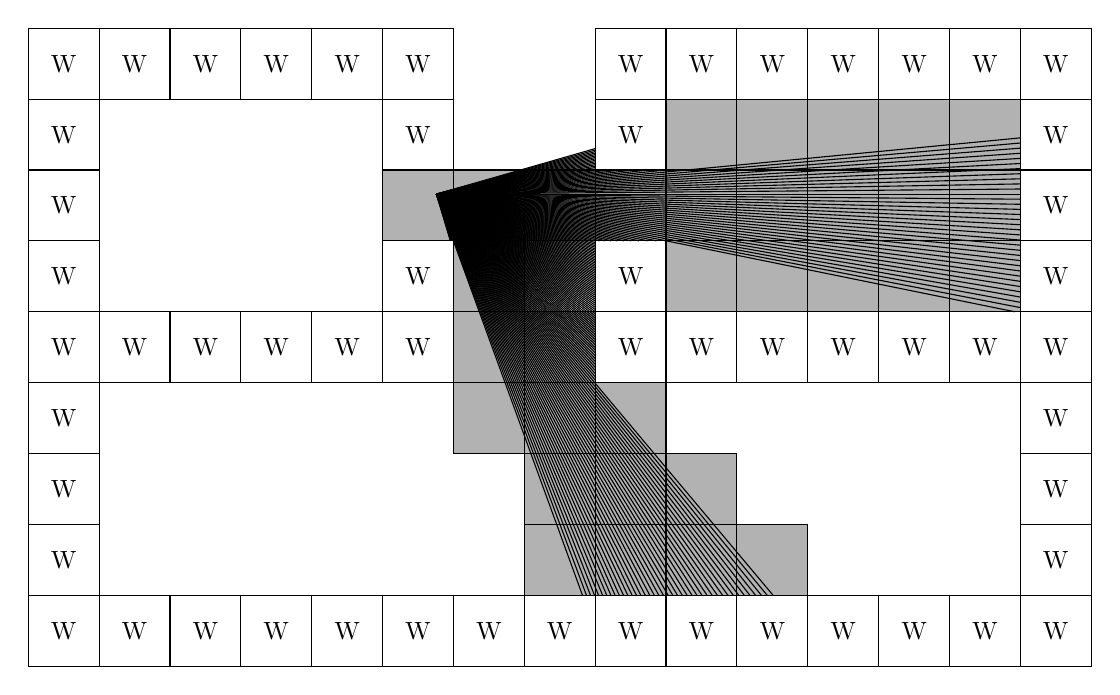
\begin{tikzpicture}[y=-1cm,scale=0.9, every node/.style={scale=0.9}]


\draw (27,55) rectangle (28,56) node[pos=.5] {W};
\draw (27,56) rectangle (28,57) node[pos=.5] {W};
\draw (27,57) rectangle (28,58) node[pos=.5] {W};
\draw (27,58) rectangle (28,59) node[pos=.5] {W};
\draw (27,59) rectangle (28,60) node[pos=.5] {W};
\draw (27,60) rectangle (28,61) node[pos=.5] {W};
\draw (27,61) rectangle (28,62) node[pos=.5] {W};
\draw (27,62) rectangle (28,63) node[pos=.5] {W};
\draw (27,63) rectangle (28,64) node[pos=.5] {W};
\draw (28,55) rectangle (29,56) node[pos=.5] {W};
\draw (28,59) rectangle (29,60) node[pos=.5] {W};
\draw (28,63) rectangle (29,64) node[pos=.5] {W};
\draw (29,55) rectangle (30,56) node[pos=.5] {W};
\draw (29,59) rectangle (30,60) node[pos=.5] {W};
\draw (29,63) rectangle (30,64) node[pos=.5] {W};
\draw (30,55) rectangle (31,56) node[pos=.5] {W};
\draw (30,59) rectangle (31,60) node[pos=.5] {W};
\draw (30,63) rectangle (31,64) node[pos=.5] {W};
\draw (31,55) rectangle (32,56) node[pos=.5] {W};
\draw (31,59) rectangle (32,60) node[pos=.5] {W};
\draw (31,63) rectangle (32,64) node[pos=.5] {W};
\draw (32,55) rectangle (33,56) node[pos=.5] {W};
\draw (32,56) rectangle (33,57) node[pos=.5] {W};
\draw (32,58) rectangle (33,59) node[pos=.5] {W};
\draw (32,59) rectangle (33,60) node[pos=.5] {W};
\draw (32,63) rectangle (33,64) node[pos=.5] {W};
\draw (33,63) rectangle (34,64) node[pos=.5] {W};
\draw (34,63) rectangle (35,64) node[pos=.5] {W};
\draw (35,55) rectangle (36,56) node[pos=.5] {W};
\draw (35,56) rectangle (36,57) node[pos=.5] {W};
\draw (35,58) rectangle (36,59) node[pos=.5] {W};
\draw (35,59) rectangle (36,60) node[pos=.5] {W};
\draw (35,63) rectangle (36,64) node[pos=.5] {W};
\draw (36,55) rectangle (37,56) node[pos=.5] {W};
\draw (36,59) rectangle (37,60) node[pos=.5] {W};
\draw (36,63) rectangle (37,64) node[pos=.5] {W};
\draw (37,55) rectangle (38,56) node[pos=.5] {W};
\draw (37,59) rectangle (38,60) node[pos=.5] {W};
\draw (37,63) rectangle (38,64) node[pos=.5] {W};
\draw (38,55) rectangle (39,56) node[pos=.5] {W};
\draw (38,59) rectangle (39,60) node[pos=.5] {W};
\draw (38,63) rectangle (39,64) node[pos=.5] {W};
\draw (39,55) rectangle (40,56) node[pos=.5] {W};
\draw (39,59) rectangle (40,60) node[pos=.5] {W};
\draw (39,63) rectangle (40,64) node[pos=.5] {W};
\draw (40,55) rectangle (41,56) node[pos=.5] {W};
\draw (40,59) rectangle (41,60) node[pos=.5] {W};
\draw (40,63) rectangle (41,64) node[pos=.5] {W};
\draw (41,55) rectangle (42,56) node[pos=.5] {W};
\draw (41,56) rectangle (42,57) node[pos=.5] {W};
\draw (41,57) rectangle (42,58) node[pos=.5] {W};
\draw (41,58) rectangle (42,59) node[pos=.5] {W};
\draw (41,59) rectangle (42,60) node[pos=.5] {W};
\draw (41,60) rectangle (42,61) node[pos=.5] {W};
\draw (41,61) rectangle (42,62) node[pos=.5] {W};
\draw (41,62) rectangle (42,63) node[pos=.5] {W};
\draw (41,63) rectangle (42,64) node[pos=.5] {W};

\filldraw[fill=black!30!white, draw=black] (32,57) rectangle (33,58);
\filldraw[fill=black!30!white, draw=black] (33,57) rectangle (34,58);
\filldraw[fill=black!30!white, draw=black] (34,57) rectangle (35,58);
\filldraw[fill=black!30!white, draw=black] (35,57) rectangle (36,58);

% Room
\filldraw[fill=black!30!white, draw=black] (36,57) rectangle (37,58);
\filldraw[fill=black!30!white, draw=black] (37,57) rectangle (38,58);
\filldraw[fill=black!30!white, draw=black] (38,57) rectangle (39,58);
\filldraw[fill=black!30!white, draw=black] (39,57) rectangle (40,58);
\filldraw[fill=black!30!white, draw=black] (40,57) rectangle (41,58);

\filldraw[fill=black!30!white, draw=black] (36,58) rectangle (37,59);
\filldraw[fill=black!30!white, draw=black] (37,58) rectangle (38,59);
\filldraw[fill=black!30!white, draw=black] (38,58) rectangle (39,59);
\filldraw[fill=black!30!white, draw=black] (39,58) rectangle (40,59);
\filldraw[fill=black!30!white, draw=black] (40,58) rectangle (41,59);

\filldraw[fill=black!30!white, draw=black] (36,56) rectangle (37,57);
\filldraw[fill=black!30!white, draw=black] (37,56) rectangle (38,57);
\filldraw[fill=black!30!white, draw=black] (38,56) rectangle (39,57);
\filldraw[fill=black!30!white, draw=black] (39,56) rectangle (40,57);
\filldraw[fill=black!30!white, draw=black] (40,56) rectangle (41,57);


\filldraw[fill=black!30!white, draw=black] (33,58) rectangle (34,59);
\filldraw[fill=black!30!white, draw=black] (33,59) rectangle (34,60);
\filldraw[fill=black!30!white, draw=black] (33,60) rectangle (34,61);
%\filldraw[fill=black!30!white, draw=black] (33,61) rectangle (34,62);
%\filldraw[fill=black!30!white, draw=black] (33,62) rectangle (34,63);
%\filldraw[fill=black!30!white, draw=black] (34,58) rectangle (35,59);
\filldraw[fill=black!30!white, draw=black] (34,59) rectangle (35,60);
\filldraw[fill=black!30!white, draw=black] (34,60) rectangle (35,61);
\filldraw[fill=black!30!white, draw=black] (34,61) rectangle (35,62);
\filldraw[fill=black!30!white, draw=black] (34,62) rectangle (35,63);

% Triangle
\filldraw[fill=black!30!white, draw=black] (35,60) rectangle (36,61);

\filldraw[fill=black!30!white, draw=black] (35,61) rectangle (36,62);
\filldraw[fill=black!30!white, draw=black] (36,61) rectangle (37,62);

\filldraw[fill=black!30!white, draw=black] (35,62) rectangle (36,63);
\filldraw[fill=black!30!white, draw=black] (36,62) rectangle (37,63);
\filldraw[fill=black!30!white, draw=black] (37,62) rectangle (38,63);

\draw[thin,black] (32.759998,57.340000) -- (35.000000,56.697712);
\draw[thin,black] (32.759998,57.340000) -- (35.000000,56.718815);
\draw[thin,black] (32.759998,57.340000) -- (35.000000,56.739815);
\draw[thin,black] (32.759998,57.340000) -- (35.000000,56.760712);
\draw[thin,black] (32.759998,57.340000) -- (35.000000,56.781525);
\draw[thin,black] (32.759998,57.340000) -- (35.000000,56.802242);
\draw[thin,black] (32.759998,57.340000) -- (35.000000,56.822868);
\draw[thin,black] (32.759998,57.340000) -- (35.000000,56.843414);
\draw[thin,black] (32.759998,57.340000) -- (35.000000,56.863884);
\draw[thin,black] (32.759998,57.340000) -- (35.000000,56.884285);
\draw[thin,black] (32.759998,57.340000) -- (35.000000,56.904602);
\draw[thin,black] (32.759998,57.340000) -- (35.000000,56.924854);
\draw[thin,black] (32.759998,57.340000) -- (35.000000,56.945038);
\draw[thin,black] (32.759998,57.340000) -- (35.000000,56.965164);
\draw[thin,black] (32.759998,57.340000) -- (35.000000,56.985229);
\draw[thin,black] (32.759998,57.340000) -- (35.035076,57.000000);
\draw[thin,black] (32.759998,57.340000) -- (35.179306,57.000000);
\draw[thin,black] (32.759998,57.340000) -- (35.342648,57.000000);
\draw[thin,black] (32.759998,57.340000) -- (35.529148,57.000000);
\draw[thin,black] (32.759998,57.340000) -- (35.744217,57.000000);
\draw[thin,black] (32.759998,57.340000) -- (35.994972,57.000000);
\draw[thin,black] (32.759998,57.340000) -- (41.000000,56.546600);
\draw[thin,black] (32.759998,57.340000) -- (41.000000,56.619114);
\draw[thin,black] (32.759998,57.340000) -- (41.000000,56.691517);
\draw[thin,black] (32.759998,57.340000) -- (41.000000,56.763821);
\draw[thin,black] (32.759998,57.340000) -- (41.000000,56.836033);
\draw[thin,black] (32.759998,57.340000) -- (41.000000,56.908173);
\draw[thin,black] (32.759998,57.340000) -- (41.000000,56.980244);
\draw[thin,black] (32.759998,57.340000) -- (41.000000,57.052261);
\draw[thin,black] (32.759998,57.340000) -- (41.000000,57.124237);
\draw[thin,black] (32.759998,57.340000) -- (41.000000,57.196175);
\draw[thin,black] (32.759998,57.340000) -- (41.000000,57.268093);
\draw[thin,black] (32.759998,57.340000) -- (41.000000,57.340000);
\draw[thin,black] (32.759998,57.340000) -- (41.000000,57.411907);
\draw[thin,black] (32.759998,57.340000) -- (41.000000,57.483826);
\draw[thin,black] (32.759998,57.340000) -- (41.000000,57.555763);
\draw[thin,black] (32.759998,57.340000) -- (41.000000,57.627739);
\draw[thin,black] (32.759998,57.340000) -- (41.000000,57.699757);
\draw[thin,black] (32.759998,57.340000) -- (41.000000,57.771828);
\draw[thin,black] (32.759998,57.340000) -- (41.000000,57.843967);
\draw[thin,black] (32.759998,57.340000) -- (41.000000,57.916180);
\draw[thin,black] (32.759998,57.340000) -- (41.000000,57.988483);
\draw[thin,black] (32.759998,57.340000) -- (41.000000,58.060886);
\draw[thin,black] (32.759998,57.340000) -- (41.000000,58.133400);
\draw[thin,black] (32.759998,57.340000) -- (41.000000,58.206036);
\draw[thin,black] (32.759998,57.340000) -- (41.000000,58.278805);
\draw[thin,black] (32.759998,57.340000) -- (41.000000,58.351715);
\draw[thin,black] (32.759998,57.340000) -- (41.000000,58.424782);
\draw[thin,black] (32.759998,57.340000) -- (41.000000,58.498020);
\draw[thin,black] (32.759998,57.340000) -- (41.000000,58.571438);
\draw[thin,black] (32.759998,57.340000) -- (41.000000,58.645050);
\draw[thin,black] (32.759998,57.340000) -- (41.000000,58.718861);
\draw[thin,black] (32.759998,57.340000) -- (41.000000,58.792892);
\draw[thin,black] (32.759998,57.340000) -- (41.000000,58.867146);
\draw[thin,black] (32.759998,57.340000) -- (41.000000,58.941647);
\draw[thin,black] (32.759998,57.340000) -- (40.919399,59.000000);
\draw[thin,black] (32.759998,57.340000) -- (35.865154,58.000000);
\draw[thin,black] (32.759998,57.340000) -- (35.737164,58.000000);
\draw[thin,black] (32.759998,57.340000) -- (35.618862,58.000000);
\draw[thin,black] (32.759998,57.340000) -- (35.509178,58.000000);
\draw[thin,black] (32.759998,57.340000) -- (35.407204,58.000000);
\draw[thin,black] (32.759998,57.340000) -- (35.312099,58.000000);
\draw[thin,black] (32.759998,57.340000) -- (35.223228,58.000000);
\draw[thin,black] (32.759998,57.340000) -- (35.139954,58.000000);
\draw[thin,black] (32.759998,57.340000) -- (35.061760,58.000000);
\draw[thin,black] (32.759998,57.340000) -- (35.000000,58.003498);
\draw[thin,black] (32.759998,57.340000) -- (35.000000,58.024818);
\draw[thin,black] (32.759998,57.340000) -- (35.000000,58.046249);
\draw[thin,black] (32.759998,57.340000) -- (35.000000,58.067799);
\draw[thin,black] (32.759998,57.340000) -- (35.000000,58.089470);
\draw[thin,black] (32.759998,57.340000) -- (35.000000,58.111271);
\draw[thin,black] (32.759998,57.340000) -- (35.000000,58.133202);
\draw[thin,black] (32.759998,57.340000) -- (35.000000,58.155266);
\draw[thin,black] (32.759998,57.340000) -- (35.000000,58.177475);
\draw[thin,black] (32.759998,57.340000) -- (35.000000,58.199829);
\draw[thin,black] (32.759998,57.340000) -- (35.000000,58.222332);
\draw[thin,black] (32.759998,57.340000) -- (35.000000,58.244991);
\draw[thin,black] (32.759998,57.340000) -- (35.000000,58.267807);
\draw[thin,black] (32.759998,57.340000) -- (35.000000,58.290791);
\draw[thin,black] (32.759998,57.340000) -- (35.000000,58.313950);
\draw[thin,black] (32.759998,57.340000) -- (35.000000,58.337280);
\draw[thin,black] (32.759998,57.340000) -- (35.000000,58.360794);
\draw[thin,black] (32.759998,57.340000) -- (35.000000,58.384499);
\draw[thin,black] (32.759998,57.340000) -- (35.000000,58.408390);
\draw[thin,black] (32.759998,57.340000) -- (35.000000,58.432484);
\draw[thin,black] (32.759998,57.340000) -- (35.000000,58.456787);
\draw[thin,black] (32.759998,57.340000) -- (35.000000,58.481300);
\draw[thin,black] (32.759998,57.340000) -- (35.000000,58.506027);
\draw[thin,black] (32.759998,57.340000) -- (35.000000,58.530987);
\draw[thin,black] (32.759998,57.340000) -- (35.000000,58.556183);
\draw[thin,black] (32.759998,57.340000) -- (35.000000,58.581608);
\draw[thin,black] (32.759998,57.340000) -- (35.000000,58.607285);
\draw[thin,black] (32.759998,57.340000) -- (35.000000,58.633221);
\draw[thin,black] (32.759998,57.340000) -- (35.000000,58.659416);
\draw[thin,black] (32.759998,57.340000) -- (35.000000,58.685879);
\draw[thin,black] (32.759998,57.340000) -- (35.000000,58.712627);
\draw[thin,black] (32.759998,57.340000) -- (35.000000,58.739658);
\draw[thin,black] (32.759998,57.340000) -- (35.000000,58.766991);
\draw[thin,black] (32.759998,57.340000) -- (35.000000,58.794624);
\draw[thin,black] (32.759998,57.340000) -- (35.000000,58.822567);
\draw[thin,black] (32.759998,57.340000) -- (35.000000,58.850845);
\draw[thin,black] (32.759998,57.340000) -- (35.000000,58.879452);
\draw[thin,black] (32.759998,57.340000) -- (35.000000,58.908405);
\draw[thin,black] (32.759998,57.340000) -- (35.000000,58.937721);
\draw[thin,black] (32.759998,57.340000) -- (35.000000,58.967392);
\draw[thin,black] (32.759998,57.340000) -- (35.000000,58.997452);
\draw[thin,black] (32.759998,57.340000) -- (35.000000,59.027897);
\draw[thin,black] (32.759998,57.340000) -- (35.000000,59.058746);
\draw[thin,black] (32.759998,57.340000) -- (35.000000,59.090012);
\draw[thin,black] (32.759998,57.340000) -- (35.000000,59.121704);
\draw[thin,black] (32.759998,57.340000) -- (35.000000,59.153843);
\draw[thin,black] (32.759998,57.340000) -- (35.000000,59.186440);
\draw[thin,black] (32.759998,57.340000) -- (35.000000,59.219505);
\draw[thin,black] (32.759998,57.340000) -- (35.000000,59.253059);
\draw[thin,black] (32.759998,57.340000) -- (35.000000,59.287125);
\draw[thin,black] (32.759998,57.340000) -- (35.000000,59.321701);
\draw[thin,black] (32.759998,57.340000) -- (35.000000,59.356819);
\draw[thin,black] (32.759998,57.340000) -- (35.000000,59.392494);
\draw[thin,black] (32.759998,57.340000) -- (35.000000,59.428741);
\draw[thin,black] (32.759998,57.340000) -- (35.000000,59.465588);
\draw[thin,black] (32.759998,57.340000) -- (35.000000,59.503048);
\draw[thin,black] (32.759998,57.340000) -- (35.000000,59.541145);
\draw[thin,black] (32.759998,57.340000) -- (35.000000,59.579899);
\draw[thin,black] (32.759998,57.340000) -- (35.000000,59.619339);
\draw[thin,black] (32.759998,57.340000) -- (35.000000,59.659481);
\draw[thin,black] (32.759998,57.340000) -- (35.000000,59.700356);
\draw[thin,black] (32.759998,57.340000) -- (35.000000,59.741989);
\draw[thin,black] (32.759998,57.340000) -- (35.000000,59.784412);
\draw[thin,black] (32.759998,57.340000) -- (35.000000,59.827652);
\draw[thin,black] (32.759998,57.340000) -- (35.000000,59.871735);
\draw[thin,black] (32.759998,57.340000) -- (35.000000,59.916695);
\draw[thin,black] (32.759998,57.340000) -- (35.000000,59.962570);
\draw[thin,black] (32.759998,57.340000) -- (37.509548,63.000000);
\draw[thin,black] (32.759998,57.340000) -- (37.425987,63.000000);
\draw[thin,black] (32.759998,57.340000) -- (37.343620,63.000000);
\draw[thin,black] (32.759998,57.340000) -- (37.262413,63.000000);
\draw[thin,black] (32.759998,57.340000) -- (37.182316,63.000000);
\draw[thin,black] (32.759998,57.340000) -- (37.103313,63.000000);
\draw[thin,black] (32.759998,57.340000) -- (37.025356,63.000000);
\draw[thin,black] (32.759998,57.340000) -- (36.948418,63.000000);
\draw[thin,black] (32.759998,57.340000) -- (36.872471,63.000000);
\draw[thin,black] (32.759998,57.340000) -- (36.797478,63.000000);
\draw[thin,black] (32.759998,57.340000) -- (36.723412,63.000000);
\draw[thin,black] (32.759998,57.340000) -- (36.650246,63.000000);
\draw[thin,black] (32.759998,57.340000) -- (36.577953,63.000000);
\draw[thin,black] (32.759998,57.340000) -- (36.506508,63.000000);
\draw[thin,black] (32.759998,57.340000) -- (36.435883,63.000000);
\draw[thin,black] (32.759998,57.340000) -- (36.366051,63.000000);
\draw[thin,black] (32.759998,57.340000) -- (36.296993,63.000000);
\draw[thin,black] (32.759998,57.340000) -- (36.228683,63.000000);
\draw[thin,black] (32.759998,57.340000) -- (36.161102,63.000000);
\draw[thin,black] (32.759998,57.340000) -- (36.094227,63.000000);
\draw[thin,black] (32.759998,57.340000) -- (36.028034,63.000000);
\draw[thin,black] (32.759998,57.340000) -- (35.962505,63.000000);
\draw[thin,black] (32.759998,57.340000) -- (35.897621,63.000000);
\draw[thin,black] (32.759998,57.340000) -- (35.833363,63.000000);
\draw[thin,black] (32.759998,57.340000) -- (35.769703,63.000000);
\draw[thin,black] (32.759998,57.340000) -- (35.706638,63.000000);
\draw[thin,black] (32.759998,57.340000) -- (35.644142,63.000000);
\draw[thin,black] (32.759998,57.340000) -- (35.582203,63.000000);
\draw[thin,black] (32.759998,57.340000) -- (35.520794,63.000000);
\draw[thin,black] (32.759998,57.340000) -- (35.459911,63.000000);
\draw[thin,black] (32.759998,57.340000) -- (35.399529,63.000000);
\draw[thin,black] (32.759998,57.340000) -- (35.339642,63.000000);
\draw[thin,black] (32.759998,57.340000) -- (35.280224,63.000000);
\draw[thin,black] (32.759998,57.340000) -- (35.221268,63.000000);
\draw[thin,black] (32.759998,57.340000) -- (35.162758,63.000000);
\draw[thin,black] (32.759998,57.340000) -- (35.104675,63.000000);
\draw[thin,black] (32.759998,57.340000) -- (35.047016,63.000000);
\draw[thin,black] (32.759998,57.340000) -- (34.989761,63.000000);
\draw[thin,black] (32.759998,57.340000) -- (34.932899,63.000000);
\draw[thin,black] (32.759998,57.340000) -- (34.876415,63.000000);
\draw[thin,black] (32.759998,57.340000) -- (34.820301,63.000000);
\draw[thin,black] (32.759998,57.340000) -- (32.993740,58.000000);
\draw[thin,black] (32.759998,57.340000) -- (32.987278,58.000000);
\draw[thin,black] (32.759998,57.340000) -- (32.980858,58.000000);
\draw[thin,black] (32.759998,57.340000) -- (32.974472,58.000000);
\draw[thin,black] (32.759998,57.340000) -- (32.968121,58.000000);
\draw[thin,black] (32.759998,57.340000) -- (32.961807,58.000000);
\draw[thin,black] (32.759998,57.340000) -- (32.955524,58.000000);
\end{tikzpicture}

 \caption{Ray cast and visible spots.} 
\end{figure}

\par
MAXVISABLE=50\\
\par


Note that the engine does not place things vertically. They are always centered vertically. The artists cleverly drew the sprites not centered vertically but at the bottom of each images. This allows for a non-expensive perspective effect even though all sprites are vertically aligned.
\par
\begin{figure}[H]
 \centering
 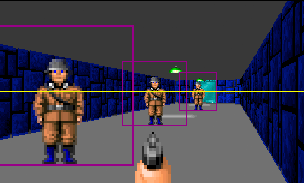
\includegraphics[width=\textwidth]{imgs/drawing_things.png}
\end{figure}
\par


  \begin{figure}[H]
\centering
 
 \caption{3D Rendere Phase 1: Backed lights} \label{fig:backee_lights}
 \end{figure}


\par
Since wall and sprites are all in the same referencial (64x64), it is easy to clip: For each column just compare the heigh from the occlusion array to the height of the thing:\\
\par
  \begin{minipage}{.5\textwidth}
     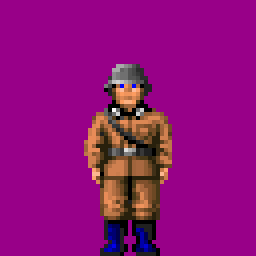
\includegraphics[width=\textwidth]{imgs/guard_sprite.png}
  \end{minipage}
   \begin{minipage}{.5\textwidth} 
     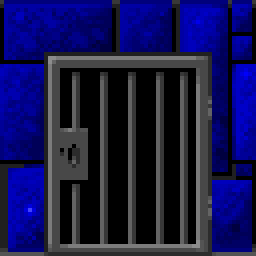
\includegraphics[width=\textwidth]{imgs/wall_texturw.png} 
   \end{minipage}

\par

  \begin{minipage}{.5\textwidth} 
     
\includegraphics[width=\textwidth]{imgs/sprite_food.png} 
   \end{minipage}
  \begin{minipage}{.5\textwidth} 
     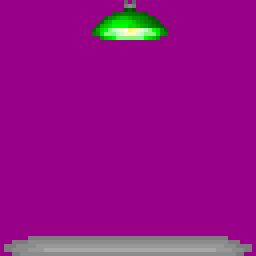
\includegraphics[width=\textwidth]{imgs/light_sprite.png}
   \end{minipage}

\par

Trivia: The sprites with a lot of transparency (such as the food and the lamp shown previously) would later turn out a major fillrate issue with hardware accelerated renderer for the iOS port:

\begin{fancyquotes}
Wolfenstein (and Doom) originally drew the characters as sparse stretched columns of solid pixels (vertical instead of horizontal for efficiency in interleaved planar mode-X VGA), but OpenGL versions need to generate a square texture with transparent pixels.  Typically this is then drawn by either alpha blending or alpha testing a big quad that is mostly empty space.  You could play through several early levels of Wolf without this being a problem, but in later levels there are often large fields of dozens of items that stack up to enough overdraw to max out the GPU and drop the framerate to 20 fps.  The solution is to bound the solid pixels in the texture and only draw that restricted area, which solves the problem with most items, but Wolf has a few different heavily used ceiling lamp textures that have a small lamp at the top and a thin but full width shadow at the bottom.  A single bounds doesn't exclude many texels, so I wound up including two bounds, which made them render many times faster. 
\bigskip \\
\textbf{John Carmack - Programmer}
 \end{fancyquotes}

TODO: Elaborate on drawing routines which uncompresse sprites on the fly.

















\subsection{Drawing weapon}
Drawing the weapon at the bottom is very straight forward. It just uses the precompiled scalar with no clipping. Nothing much to say abou that :/!\\













\subsection{I.A: State Machines}
The 3D engine not only draw things, it also allows all objects to "think". 
Closely tied to sound system: Enemy responding to audio clue are deemed smarter!!\\
Defined in WL\_ACT2.c\\
Normal, standing guard\\
Walking guard\\
Deaf guard\\

Planes:
=Ambush tile: enemy placed ohere are deaf to all attacks (normal enemy responds immediately to sound).\\
An ambush tile-affected enemy is not blind but attack playe but won't react to dead soldiers or dogs.\\
\par
How does sound travel between areas ? If a door is open, and a fire is shot, enemies in other room will come.\\
areabyplayer connect players\\
\par
I/A also faked with map waypoint for patrolling.\\



\section{Heathbeats}
VGA: 70Hz
audio: Depends on quality, three levels of fidelity.